\documentclass[a4paper,14pt,oneside,openany]{memoir}

%%% Задаем поля, отступы и межстрочный интервал %%%

\usepackage[left=30mm, right=15mm, top=20mm, bottom=20mm]{geometry} % Пакет geometry с аргументами для определения полей
\pagestyle{plain} % Убираем стандарные для данного класса верхние колонтитулы с заголовком текущей главы, оставляем только номер страницы снизу по центру
\parindent=1.25cm % Абзацный отступ 1.25 см, приблизительно равно пяти знакам, как по ГОСТ
\usepackage{indentfirst} % Добавляем отступ к первому абзацу
%\linespread{1.3} % Межстрочный интервал (наиболее близко к вордовскому полуторному) - тут вместо этого используется команда OnehalfSpacing*

%%% Задаем языковые параметры и шрифт %%%

\usepackage[english, russian]{babel}                % Настройки для русского языка как основного в тексте
\babelfont{rm}{Times New Roman}                     % TMR в качестве базового roman-щрифта

%%% Задаем стиль заголовков и подзаголовков в тексте %%%

\setsecnumdepth{subsection} % Номера разделов считать до третьего уровня включительно, т.е. нумеруются только главы, секции, подсекции
\renewcommand*{\chapterheadstart}{} % Переопределяем команду, задающую отступ над заголовком, чтобы отступа не было
\renewcommand*{\printchaptername}{} % Переопределяем команду, печатающую слово "Глава", чтобы оно не печалось
%\renewcommand*{\printchapternum}{} % То же самое для номера главы - тут не надо, номер главы оставляем
\renewcommand*{\chapnumfont}{\normalfont\bfseries} % Меняем стиль шрифта для номера главы: нормальный размер, полужирный
\renewcommand*{\afterchapternum}{\hspace{1em}} % Меняем разделитель между номером главы и названием
\renewcommand*{\printchaptertitle}{\normalfont\bfseries\centering} % Меняем стиль написания для заголовка главы: нормальный размер, полужирный, центрированный, заглавными буквами
\setbeforesecskip{20pt} % Задаем отступ перед заголовком секции
\setaftersecskip{20pt} % Ставим такой же отступ после заголовка секции
\setsecheadstyle{\raggedright\normalfont\bfseries\centering} % Меняем стиль написания для заголовка секции: выравнивание по правому краю без переносов, нормальный размер, полужирный
\setbeforesubsecskip{20pt} % Задаем отступ перед заголовком подсекции
\setaftersubsecskip{20pt} % Ставим такой же отступ после заголовка подсекции
\setsubsecheadstyle{\raggedright\normalfont\bfseries\itshape\centering}  % Меняем стиль написания для заголовка подсекции: выравнивание по правому краю без переносов, нормальный размер, полужирный

%%% Задаем параметры оглавления %%%

% \addto\captionsrussian{\renewcommand\contentsname{Содержание}} % Меняем слово "Оглавление" на "Содержание"
\setrmarg{2.55em plus1fil} % Запрещаем переносы слов в оглавлении
%\setlength{\cftbeforechapterskip}{0pt} % Эта команда убирает интервал между заголовками глав - тут не надо, так красивее смотрится
\renewcommand{\aftertoctitle}{\afterchaptertitle \vspace{-\cftbeforechapterskip}} % Делаем отступ между словом "Содержание" и первой строкой таким же, как у заголовков глав
%\renewcommand*{\chapternumberline}[1]{} % Делаем так, чтобы номер главы не печатался - тут не надо
\renewcommand*{\cftchapternumwidth}{1.5em} % Ставим подходящий по размеру разделитель между номером главы и самим заголовком
\renewcommand*{\cftchapterfont}{\normalfont} % Названия глав обычным шрифтом заглавными буквами
\renewcommand*{\cftchapterpagefont}{\normalfont} % Номера страниц обычным шрифтом
\renewcommand*{\cftchapterdotsep}{\cftdotsep} % Делаем точки до номера страницы после названий глав
\renewcommand*{\cftdotsep}{1} % Задаем расстояние между точками
\renewcommand*{\cftchapterleader}{\cftdotfill{\cftchapterdotsep}} % Делаем точки стандартной формы (по умолчанию они "жирные")
\maxtocdepth{subsection} % В оглавление попадают только разделы первыхтрех уровней: главы, секции и подсекции

%%% Выравнивание и переносы %%%

%% http://tex.stackexchange.com/questions/241343/what-is-the-meaning-of-fussy-sloppy-emergencystretch-tolerance-hbadness
%% http://www.latex-community.org/forum/viewtopic.php?p=70342#p70342
\tolerance 1414
\hbadness 1414
\emergencystretch 1.5em                             % В случае проблем регулировать в первую очередь
\hfuzz 0.3pt
\vfuzz \hfuzz
%\dbottom
%\sloppy                                            % Избавляемся от переполнений
\clubpenalty=10000                                  % Запрещаем разрыв страницы после первой строки абзаца
\widowpenalty=10000                                 % Запрещаем разрыв страницы после последней строки абзаца
\brokenpenalty=4991                                 % Ограничение на разрыв страницы, если строка заканчивается переносом

%%% Объясняем компилятору, какие буквы русского алфавита можно использовать в перечислениях (подрисунках и нумерованных списках) %%%
%%% По ГОСТ нельзя использовать буквы ё, з, й, о, ч, ь, ы, ъ %%%
%%% Здесь также переопределены заглавные буквы, хотя в принципе они в документе не используются %%%

\makeatletter
    \def\russian@Alph#1{\ifcase#1\or
       А\or Б\or В\or Г\or Д\or Е\or Ж\or
       И\or К\or Л\or М\or Н\or
       П\or Р\or С\or Т\or У\or Ф\or Х\or
       Ц\or Ш\or Щ\or Э\or Ю\or Я\else\xpg@ill@value{#1}{russian@Alph}\fi}
    \def\russian@alph#1{\ifcase#1\or
       а\or б\or в\or г\or д\or е\or ж\or
       и\or к\or л\or м\or н\or
       п\or р\or с\or т\or у\or ф\or х\or
       ц\or ш\or щ\or э\or ю\or я\else\xpg@ill@value{#1}{russian@alph}\fi}
\makeatother

%%% Задаем параметры оформления рисунков и таблиц %%%

\usepackage{graphicx, caption, subcaption} % Подгружаем пакеты для работы с графикой и настройки подписей
\graphicspath{{images/}} % Определяем папку с рисунками
\captionsetup[figure]{font=small, width=\textwidth, name=Рисунок, justification=centering} % Задаем параметры подписей к рисункам: маленький шрифт (в данном случае 12pt), ширина равна ширине текста, полнотекстовая надпись "Рисунок", выравнивание по центру
\captionsetup[subfigure]{font=small} % Индексы подрисунков а), б) и так далее тоже шрифтом 12pt (по умолчанию делает еще меньше)
\captionsetup[table]{singlelinecheck=false,font=small,width=\textwidth,justification=justified} % Задаем параметры подписей к таблицам: запрещаем переносы, маленький шрифт (в данном случае 12pt), ширина равна ширине текста, выравнивание по ширине
\captiondelim{---} % Разделителем между номером рисунка/таблицы и текстом в подписи является длинное тире
\setkeys{Gin}{width=\textwidth} % По умолчанию размер всех добавляемых рисунков будет подгоняться под ширину текста
\renewcommand{\thesubfigure}{\asbuk{subfigure}} % Нумерация подрисунков строчными буквами кириллицы
%\setlength{\abovecaptionskip}{0pt} % Отбивка над подписью - тут не меняем
%\setlength{\belowcaptionskip}{0pt} % Отбивка под подписью - тут не меняем
\usepackage{float}
\usepackage[section]{placeins} % Объекты типа float (рисунки/таблицы) не вылезают за границы секциии, в которой они объявлены


%%% Задаем параметры ссылок и гиперссылок %%% 

\usepackage{hyperref}                               % Подгружаем нужный пакет
\hypersetup{
    colorlinks=true,                                % Все ссылки и гиперссылки цветные
    linktoc=all,                                    % В оглавлении ссылки подключатся для всех отображаемых уровней
    linktocpage=true,                               % Ссылка - только номер страницы, а не весь заголовок (так выглядит аккуратнее)
    linkcolor=black,                                  % Цвет ссылок и гиперссылок - красный
    citecolor=black,                                 % Цвет цитировний - красный
    urlcolor=black
}

%%% Настраиваем отображение списков %%%

\usepackage{enumitem}                               % Подгружаем пакет для гибкой настройки списков
\renewcommand*{\labelitemi}{\textbullet}        % В ненумерованных списках для пунктов используем короткое тире
\makeatletter
    \AddEnumerateCounter{\asbuk}{\russian@alph}     % Объясняем пакету enumitem, как использовать asbuk
\makeatother
\renewcommand{\labelenumii}{\asbuk{enumii})}        % Кириллица для второго уровня нумерации
\renewcommand{\labelenumiii}{\arabic{enumiii})}     % Арабские цифры для третьего уровня нумерации
\setlist[enumerate]{wide=\parindent}
\setlist[itemize]{wide=\parindent}
\setlist{noitemsep, topsep=0pt, leftmargin=*}                  % Убираем интервалы между пунками одного уровня в списке
\setlist[1]{labelindent=\parindent}                 % Отступ у пунктов списка равен абзацному отступу
\setlist[2]{leftmargin=\parindent}                  % Плюс еще один такой же отступ для следующего уровня
\setlist[3]{leftmargin=\parindent}                  % И еще один для третьего уровня

%%% Счетчики для нумерации объектов %%%

\counterwithin{figure}{chapter}                    
\counterwithout{equation}{chapter}                  % Сквозная нумерация математических выражений по документу
\counterwithout{table}{chapter}                     % Сквозная нумерация таблиц по документу

%%% Реализация библиографии пакетами biblatex и biblatex-gost с использованием движка biber %%%

\usepackage{csquotes} % Пакет для оформления сложных блоков цитирования (biblatex рекомендует его подключать)
\usepackage[%
backend=biber,                                      % Движок
bibencoding=utf8,                                   % Кодировка bib-файла
sorting=none,                                       % Настройка сортировки списка литературы
style=gost-numeric,                                 % Стиль цитирования и библиографии по ГОСТ
language=auto,                                      % Язык для каждой библиографической записи задается отдельно
autolang=other,                                     % Поддержка многоязычной библиографии
sortcites=none,                                     % Если в квадратных скобках несколько ссылок, то отображаться будут отсортированно
movenames=false,                                    % Не перемещать имена, они всегда в начале библиографической записи
maxnames=5,                                         % Максимальное отображаемое число авторов
minnames=3,                                         % До скольки сокращать число авторов, если их больше максимума
doi=false,                                          % Не отображать ссылки на DOI
isbn=false,                                         % Не показывать ISBN, ISSN, ISRN
]{biblatex}

\defbibenvironment{bibliography}
  {\enumerate[wide=\parindent]}
  {\endenumerate}
  {\item}

\DeclareDelimFormat{bibinitdelim}{}                 % Убираем пробел между инициалами (Иванов И.И. вместо Иванов И. И.)

\renewcommand*{\mkgostheading}[1]{#1}

\addbibresource{biba.bib}                           % Определяем файл с библиографией

%%% Скрипт, который автоматически подбирает язык (и, следовательно, формат) для каждой библиографической записи %%%
%%% Если в названии работы есть кириллица - меняем значение поля langid на russian %%%
%%% Все оставшиеся пустые места в поле langid заменяем на english %%%

\DeclareSourcemap{
  \maps[datatype=bibtex]{
    \map{
        \step[fieldsource=title, match=\regexp{^\P{Cyrillic}*\p{Cyrillic}.*}, final]
        \step[fieldset=langid, fieldvalue={russian}]
    }
    \map{
        \step[fieldset=langid, fieldvalue={english}]
    }
  }
}


%%% Прочие пакеты для расширения функционала %%%

\usepackage{longtable,ltcaption}                    % Длинные таблицы
\usepackage{multirow,makecell}                      % Улучшенное форматирование таблиц
\usepackage{booktabs}                               % Еще один пакет для красивых таблиц
\usepackage{soulutf8}                               % Поддержка переносоустойчивых подчёркиваний и зачёркиваний
\usepackage{icomma}                                 % Запятая в десятичных дробях
\usepackage{hyphenat}                               % Для красивых переносов
\usepackage{textcomp}                               % Поддержка "сложных" печатных символов типа значков иены, копирайта и т.д.
\usepackage[version=4]{mhchem}                      % Красивые химические уравнения
\usepackage{amsmath}                                % Усовершенствование отображения математических выражений 

%%% Вставляем по очереди все содержательные части документа %%%

\begin{document}

\thispagestyle{empty}

\begin{center}
    \small Автономная некоммерческая образовательная организация \\
    высшего образования \\
    \uppercase{\textbf{<<Научно-технологический университет <<Сириус>>}}

    \vspace{20pt}

    \small Научный центр информационных технологий и искусственного интеллекта \\
    направление <<Математическое моделирование в биомедицине и геофизике>>

    \vspace{20pt}
    
\end{center}

\noindent
\begin{tabularx}{\textwidth}{Xl}
    & К ЗАЩИТЕ ДОПУСТИТЬ \\
    \addlinespace[2mm] 
    & \small Научный руководитель направления \\
    & \small <<Математическое моделирование в \\
    & \small биомедицине и геофизике>> \\
    & \small д.ф.-м.н., профессор, чл.-корр. РАН \\
    & \small \underline{\hspace{3cm}} Ю.В. Василевский \\
    & \small «\underline{\hspace{1cm}}» \underline{\hspace{2cm}} 20\underline{\hspace{1cm}} г. \\
\end{tabularx}

\vspace{20pt}

\begin{center}
    \uppercase{Оптимизация модели кровотока для диагностики стенозов коронарных артерий} \\  

    \vspace{20pt}

    \small Магистерская диссертация  \\
    
    \small по направлению подготовки 01.04.02 Прикладная математика и информатика \\
    
    \small (направленность (профиль) <<Математическое моделирование в биомедицине и нефтегазовом инжиниринге>>)   
\end{center}

\vfill

\noindent
\begin{tabularx}{\textwidth}{@{}XX@{}}
  & \small Студент гр. М01ММ-23 \\ 
  & \small \underline{\hspace{3cm}} Д.А. Гребеников \\
  & \small «\underline{\hspace{1cm}}» \underline{\hspace{2cm}} 20\underline{\hspace{1cm}} г. \\
  & \\
  & \\
  \\
  & \small Научный руководитель \\
  & \small магистерской диссертации\\
  & \small Научный руководитель направления \\
  & \small <<Математическое моделирование в \\
  & \small биомедицине и геофизике» Научного  \\
  & \small центра информационных технологий и   \\
  & \small искусственного интеллекта, к.ф.-м.н, доцент НТУ "Сириус",  \\
  % & \small д.ф.-м.н., профессор, чл.-корр. РАН \\
  & \small \underline{\hspace{3cm}} Т.М. Гамилов \\
  & \small «\underline{\hspace{1cm}}» \underline{\hspace{2cm}} 20\underline{\hspace{1cm}} г. \\
\end{tabularx}

\vfill

\begin{center}
    \small Федеральная территория <<Сириус>>, 2025
\end{center}                                     % Титульник

\newpage % Переходим на новую страницу
 % Начинаем считать номера страниц со второй
\OnehalfSpacing* % Задаем полуторный интервал текста (в титульнике одинарный, поэтому команда стоит после него)

\setcounter{page}{4}
\chapter*{Реферат}

Выпускная квалификационная работа, X страницы, X рисунков, X источников.

ОПТИМИЗАЦИЯ МОДЕЛИ КРОВОТОКА ДЛЯ ДИАГНОСТИКИ СТЕНОЗОВ КОРОНАРНЫХ АРТЕРИЙ

Цель работы:
%услорение
Оптимизация вычислений одномерной модели кровотока для программного комплекса по поддержке принятия врачебных решений по стентированию коронарных артерий.

Результаты работы:

В рамках дипломной работы предложен и реализован метод постановки граничных условий в виде модели упругого резервуара для одномерной модели гемодинамики. Это позволяет быстрее и без потери точности оценивать фракционный резерв кровотока в коронарных артериях со стенозами. Апробация на клинических данных подтвердила эффективность метода.
   
\chapter*{Сокращения, обозначения, термины 
и определения}

В настоящей работе применяют следующие сокращения и обозначения:
\begin{itemize}

\item ФРК --- Фракционный резерв кровотока;

\item ССЗ --- Сердечно сосудистые заболевания;

\item 0D/1D --- Zero-dimensional/One-dimensional (Нольмерный/Одномерный).

\iffalse
\item AVD --- Aortic Valve Disease (Аортальный порок сердца);

\item AV-Rec --- Aortic Valve Reconstruction (Реконструкция аортального клапана);

\item CSS --- Cascading Style Sheets (Каскадные таблицы стилей);

\item DICOM --- Digital Imaging and Communications in Medicine (Цифровая обработка и передача медицинских изображений);

\item DOM --- Document Object Model (Объектная модель документа);

\item GCC --- Google Closure Compiler (Компилятор Google Closure);

\item GL --- Graphics Library (Графическая библиотека);

\item HTML --- HyperText Markup Language (Язык разметки гипертекста);

\item HTTPS --- HyperText Transfer Protocol Secure (Безопасный протокол передачи гипертекста);

\item JS --- JavaScript (Язык программирования JavaScript);

\item JSX --- JavaScript XML (Расширение синтаксиса JavaScript для использования XML/HTML);

\item КТ --- Компьютерная томография;

\item MVP --- Minimum Viable Product (Минимально жизнеспособный продукт);

\item СППВР --- Система поддержки принятия врачебных решений;

\item UI --- User Interface (Пользовательский интерфейс);

\item XML --- eXtensible Markup Language (Расширяемый язык разметки);

\item шейдеры —-- это программы, предназначенные для выполнения на графическом процессоре, которые определяют аспекты визуализации 3D-графики, включая цвета, освещение и тени;

\item 2D/3D --- Two-dimensional/Three-dimensional (Двумерный/Трехмерный).
\fi
\end{itemize}    

\newpage

\tableofcontents*                                   % Автособираемое оглавление

\chapter*{Введение}
\addcontentsline{toc}{chapter}{Введение}
\label{ch:intro}

%Актуальность -- Проблематика -- Цель

%Сердечно сосудистые заболевания попрежнему остаются основной причиной смертнос
Cердечно-сосудистые заболевания по-прежнему остаются ведущей причиной смертности взрослого населения в развитых странах \cite{1}, что обуславливает необходимость развития математических моделей кровотока как для расчета индивидуальных рисков, так и для поддержки клинических решений. Особую актуальность данное направление приобретает в сфере инвазивных процедур, таких как стентирование коронарных артерий, где расчет фракционного резерва кровотока (ФРК) критически важен для определения необходимости хирургического вмешательства.

Однако существующие одномерные модели кровотока сталкиваются с рядом ограничений, которые препятствуют их широкому введению в клиническую практику. Во-первых, данные модели требуют значительных вычислительных ресурсов из-за сложности методов, решающих уравнения, которые описывают пульсирующий поток крови. Также важна  оперативность результатов, что особенно актуально для таких задач, как интраоперационный мониторинг или экстренная диагностика. Во-вторых, многие модели зависят от параметров, которые невозможно получить неинвазивными методами. Например, данные о локальном давлении, жёсткости стенок сосудов или периферическом сопротивлении часто требуют проведения инвазивных процедур, таких как катетеризация, что сопряжено с риском для пациента и увеличивает стоимость обследования. Кроме того, такие измерения могут быть недоступны в рутинной практике, что ограничивает применимость моделей в стандартных клинических сценариях.

Третья проблема заключается в сложности персонализации моделей под индивидуальные анатомические и физиологические особенности пациентов. Необходимость ручной настройки параметров увеличивают время подготовки модели и риск ошибок, особенно при отсутствии полного набора диагностических данных. Это делает процесс трудоёмким и малопригодным для массового использования, где ключевыми факторами остаются простота и скорость интерпретации результатов.

%Windkessel == эластичного (упругого) резервуара

Для преодоления указанных ограничений в данной работе предлагается подход, объединяющий одномерную модель коронарного кровотока с моделью эластичного (упругого) резервуара, которая заменяет ресурсоемкие вычисления в одномерной виртуальной аорте на компактную 0D модель. При данном подходе снижается количество необходимых начальных параметров при сохранении значимости результатов. Новизна работы заключается в разработке адаптивных граничных условий для одномерной модели кровотока, которые позволят облегчить проведение персонализации модели под конкретного пациента и ускорить вычисления. 

В рамках исследования предлагается решение следующих задач:
\begin{enumerate}
	\item Изучить текущие модели кровотока и использующиеся граничные условия и их параметры.
	\item Разработать персонализированные граничные условия.
	\item Разработать механизм адаптации модели под данные конкретного пациента.
	\item Проверить решение на имеющейся пациентной базе.
	\item Сравнить результаты работы моделей с виртуальной аортой и без.
\end{enumerate}


%провести литературный обзор существующих моделей коронарного кровотока и сравнительный анализ одномерной модели с граничными условиями в виде виртуальной аорты и в виде адаптивной модели эластичного резервуара. Для валидации подхода будут использованы как синтетические данные, позволяющие сравнить результаты работы модели с результатами  предыдущей модели, так и клинические данные пациентов.
% 

% цель работы - четко и  задачи для достижения цели

%\begin{enumerate}
%	\item Изучить текущие модели кротока и испольщующиеся граничные условия и их параметры.
%	\item Разработать персонализированные граничные условия с учетом опыта коллег.
%	\item Проверить решение на имеющейся пациентной базе.
%\end{enumerate}


% разработать мат модель стыковки аорты с коронарными артериями
% По мат можели реализовать чиссленный метод для расчета уравнений в узле аорты
% интегрировать модель распределения потоков в аорте в можель одномерного кровотока
% предложить механизм адаптации аорты для персонадизации модеди
% валидация на данных реальзых пациентов





%Персонализированные модели играют важную роль в биомедицинских задачах, так как они учитывают индивидуальные особенности каждого пациента. Такие модели позволяют формализовать и связать ключевые патофизиологические процессы, оценивать важные для диагностики заболевания параметры и прогнозировать результаты терапевтических или хирургических вмешательств. Однако для успешного использования моделей в клинической практике необходимо обеспечить их валидацию, автоматизацию технологической цепочки от обработки входных данных до получения результата, а также высокую скорость расчетов \cite{василевский2022персонализация}. 

%Для автоматизации такой технологической цепочки необходимо разработать систему поддержки принятия врачебных решений (СППВР). Задача разработки СППВР включает в себя не только разработку математической модели, но и создание удобного интерфейса для взаимодействия с врачами, что особенно важно для эффективного применения в клинической практике \cite{shaalan2020visualization}.

%Для успешного внедрения СППВР в клиническую практику необходимо, чтобы система удовлетворяла следующим техническим критериям: масштабируемость, развертываемость, поддерживаемость, сопровождаемость, совместимость внутренних модулей. Эти критерии распространяются и на внутренние модули системы, в том числе на интерфейс. 

%Помимо технических критериев, самым важным является практическая значимость для врачей: разрабатываемая система должна уметь эффективно решать актуальную проблему врачей. 

%В рамках данной работы было предложено проанализировать проблемы старого веб-интерфейса СППВР для операции Озаки, изучить современные подходы к созданию веб-интерфейса и реализовать новую кодовую базу на основе этих фреймворков или доработать существующую.

%Цель данной работы --- разработка пользовательского веб-интерфейса в системе поддержки принятия врачебных решений для операции Озаки с использованием современных фреймворков.

%Список задач для достижения цели:
%\begin{enumerate}
   % \item Анализ предметной области: Изучить специфику операции Озаки и определить функциональные и нефункциональные требования к системе.
   % \item Анализ проблем предыдущего решения и современных подходов к созданию клиентских веб-приложений: Оценить старый веб-интерфейс, выявить его недостатки и рассмотреть современные подходы к разработке интерфейсов.
   % \item Реализация веб-интерфейса: Описать и реализовать новую кодовую базу с использованием современных фреймворков, описать интеграцию библиотек для решения возникающих задач, обеспечить интеграцию всех компонентов системы.
%\end{enumerate}

\endinput                                     % Введение
\chapter{\MakeUppercase{Обзор литературы}}
\label{ch:chap1}

В первой главе рассматривается...

\section{По ФРК и кровотоку}
Стеноз коронарных артерий -- это патологическое сужение просвета сосудов, ответственных за кровоснабжение сердца (Рисунок {\ref*{fig:1}}). При значительно уменьшении диаметра артерии развивается ишемия миокарда, которая проявляется стенокардией, одышкой, а в критических случаях -- инфарктом. Основной причиной возникновения стенозов является атеросклероз - хроническое заболевание, при котором на внутренних стенках сосудов формируются холестериновые бляшки. Эти образования состоят из липидов, кальция и соединительной ткани. Со временем бляшки увеличиваются, нарушая кровоток, а их разрыв может спровоцировать риск тромбоза и полной закупорки сердца.

  
Стентирование -- инвазивная операция, направленная на восстановление проходимости крови в пораженной артерии. Выполняется под местной анестезией через прокол в бедренной или лучевой артерии, через который под рентген-контролем вводится катетер к сердцу. После ангиографии с контрастным веществом, выявляющей локализацию и степень стеноза, выполняется баллонная ангиопластика: миниатюрный баллон раздувается в зоне сужения, восстанавливая просвет сосуда. Затем имплантируется стент — металлический сетчатый каркас, предотвращающий рестеноз. Современные стенты с лекарственным покрытием снижают риск разрастания рубцовой ткани.


Для определения функциональной значимости стеноза перед вмешательством используется фракционный резерв кровотока (ФРК) -- гемодинамический индекс, оценивающий градиент давления до и после сужения. 

\begin{equation}\label{eq:e1}
	FFR = \frac{P_d}{P_a},
\end{equation}
где $P_d$ -- давление крови после стеноза, $P_a$ -- давление в аорте.

\begin{figure}
	\centering
	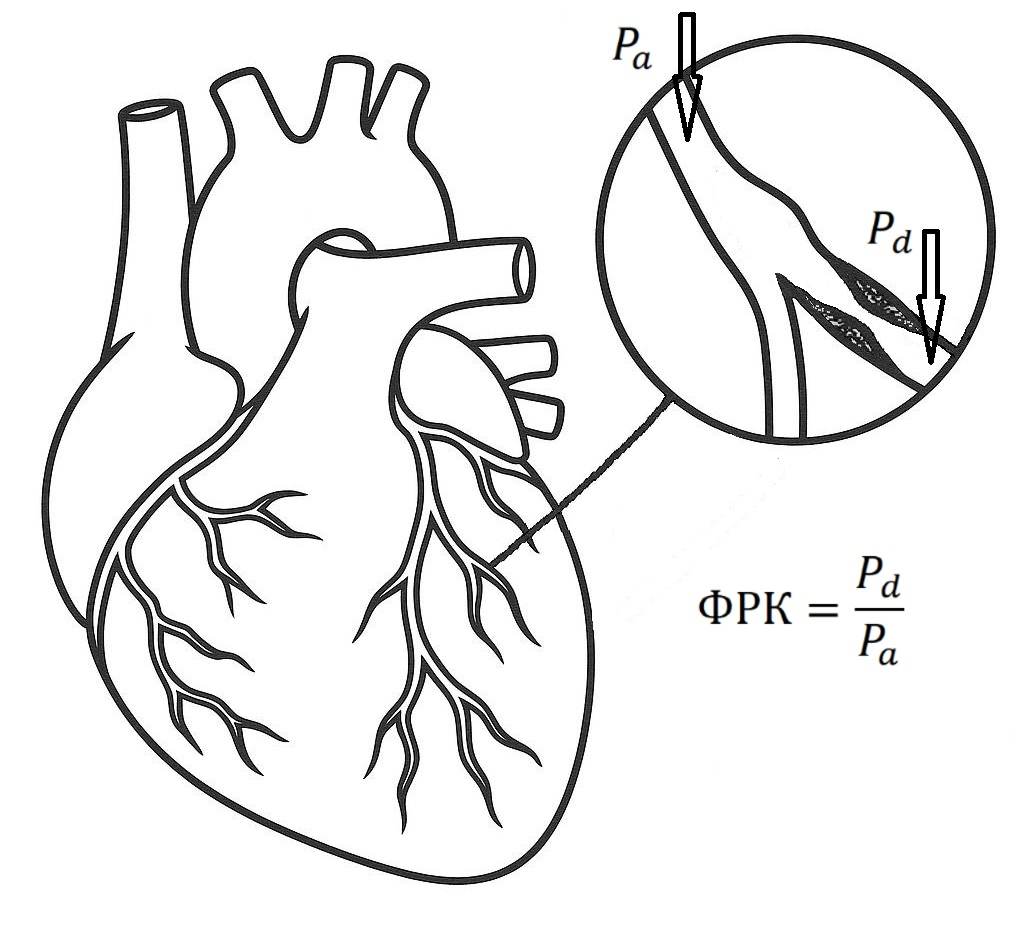
\includegraphics[]{images/chap1/FFR_dem.jpg}
	\caption{Стеноз левой коронарной артерии.}
	\label{fig:1}
\end{figure}
%\hyperref[fig:dicom]{рисунке \ref*{fig:dicom}}

ФРК помогает выявить, вызывает ли стеноз ишемию миокарда: значение ≤ 0.8 указывает на необходимость стентирования, что повышает точность отбора пациентов и снижает риск избыточных вмешательств. Для определения ФРК в медицинской практике используют инвазивные методы с использованием провокационных тестов. Введение вазодилататоров (сосудо-расширяющих препаратов), таких как аденозин или папаверин, вызывает гиперемию -- усиление кровотока, что позволяет измерить давление до и после сужения артерии с помошью специального датчика (Рисунок {\ref*{fig:2}}). Этот тонкий проводник с датчиком давления продвигается через катетер к пораженному участку артерии, регистрируя изменения в реальном времени. Ангиограмма, совмещенная с данными ФРК, визуализирует зону ишемии, обеспечивая точное планирование операции.

\begin{figure}
	\centering
	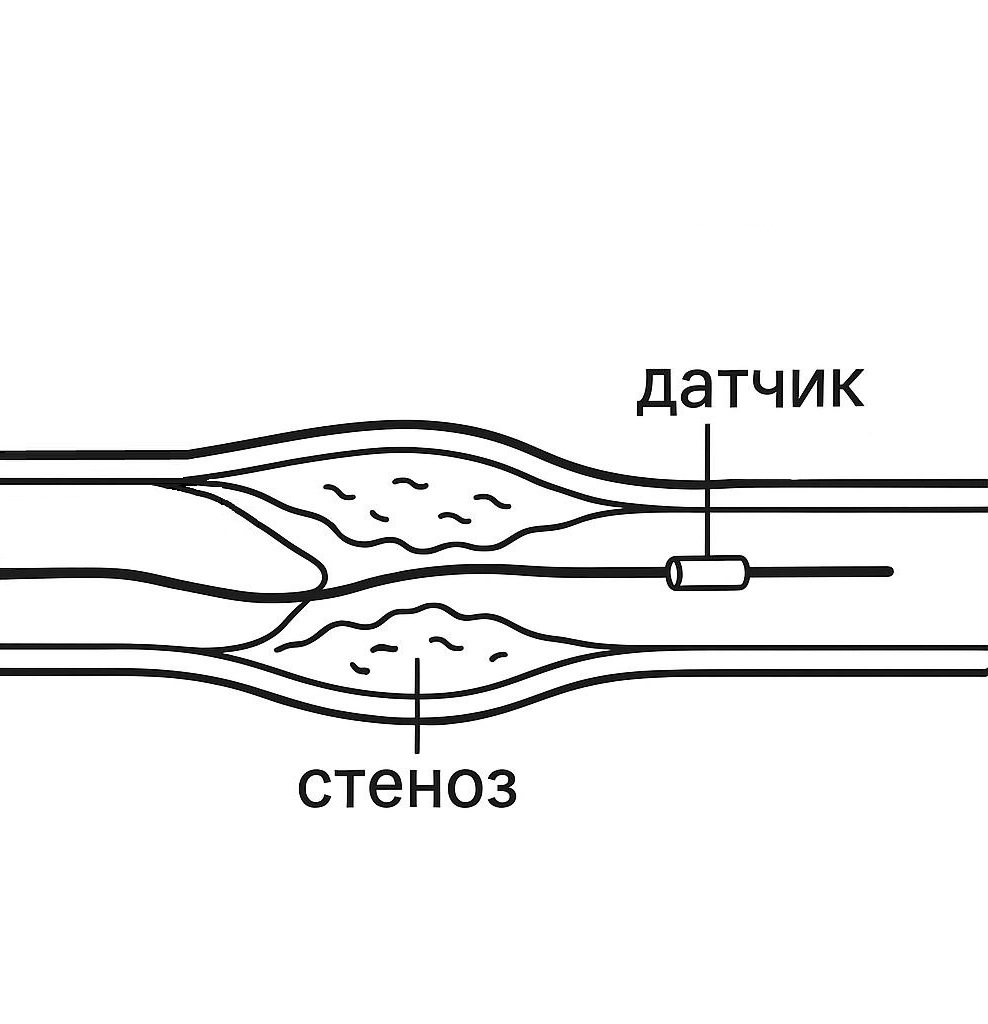
\includegraphics[]{images/chap1/pressure_wire.jpg}
	\caption{Введение катетера с датчиком давления в область стенозированного участка артерии.}
	\label{fig:2}
\end{figure}

Существует и альтернативный способ измерения ФРК -- с помощью математических моделей кровотока. Данный метод не требует инвазивного хирургического вмешательства и позволяет с некоторой погрешностью оценивать значение давления в артериях. Часто используются модели [Ссылки на модели], использующие данные компьютерной томографии (КТ), на основе которых строится 0D/3D модель коронарных артерий в которой с помощью алгоритмов гидродинамики прогнозируются характеристики тока крови.Точность таких расчетов достигает X [Ссылка на статью с точностью], что сопоставимо с инвазивным методом, но без рисков катетеризации.

Клиническая значимость ФРК:
{Согласно рекомендациям ESC/ACC, FFR <0.8 является ключевым критерием для принятия решения о реваскуляризации. Исследование FAME доказало, что FFR-ориентированная стратегия снижает риск основных сердечно-сосудистых событий (MACE) на 30\% по сравнению с ангиографическим подходом. Алгоритм включает этапы: оценка симптомов → ангиография → измерение FFR → стентирование при FFR ≤0.8.}


Ограничения ФРК:
{Несмотря на высокую точность, FFR имеет ограничения. Микрососудистая дисфункция (например, при диабете или гипертонии) может искажать результаты: в таких случаях FFR остается нормальным, но стресс-тесты выявляют ишемию из-за нарушения вазодилатации мелких сосудов. Это явление называют «диссоциацией FFR и ишемии», что требует комплексной оценки с использованием дополнительных методов (например, индекса микрососудистого сопротивления).}

Картинка : Схема микрососудистой дисфункции (сравнение здоровых и пораженных микрососудов).

\iffalse
\begin{figure}
	\centering
	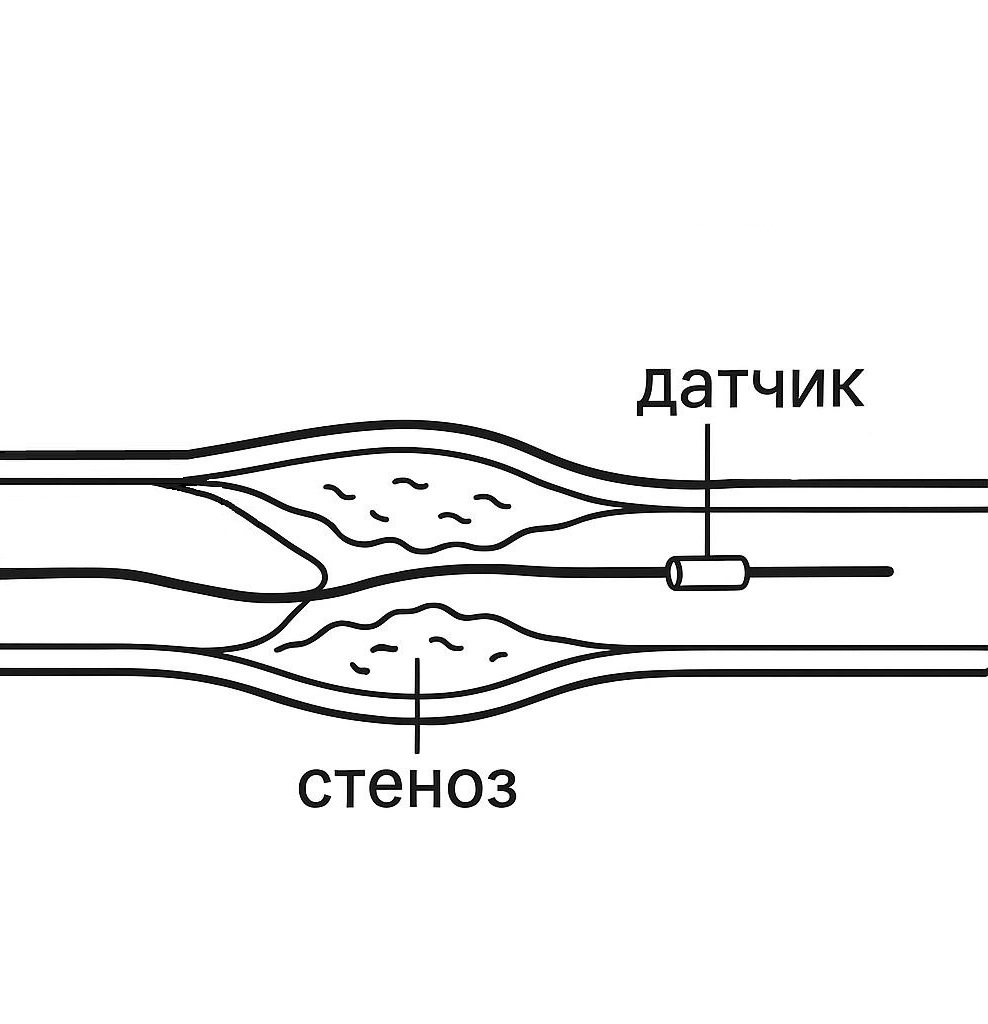
\includegraphics[]{images/chap1/pressure_wire.jpg}
	\caption{Сравнение здоровых и пораженных сосудов.}
	\label{fig:2}
\end{figure}
\fi

\section{По моделям для вычисления ФРК}
Современные модели кровотока позволяют...

% \subsection{Подсекция, в которой мы демонстрируем, как выглядят многоуровневые нумерованные списки}

%     Теперь попробуем разобраться с нумерованным списком. Его можно делать многоуровневым, при этом нам важно соблюдать формирование по ГОСТ: в подпунктах используются буквы русского алфавита (все, кроме ё, з, й, о, ч, ь, ы, ъ). Необходимое форматирование уже задано в основном файле. Выглядеть это будет так:

%     \begin{enumerate}
%         \item Первый пункт
%         \begin{enumerate}
%             \item Первый подпункт первого пункта
%             \item Второй подпункт первого пункта
%         \end{enumerate}
%         \item Второй пункт
%         \begin{enumerate}
%             \item Первый подпункт второго пункта
%             \item Второй подпункт второго пункта
%             \begin{enumerate}
%                 \item Это уже подпункт третьего уровня
%                 \item Сделаем еще один подпункт третьего уровня. Он будет достаточно большим, чтобы показать, как текст в нумерованном списке переносится на следующую строку
%             \end{enumerate}
%             \item Третий подпункт
%         \end{enumerate}
%     \end{enumerate}

% \section{Метки и ссылки}

% В \LaTeX{}е достаточно большие возможности для создания различного рода ссылок в тексте. Можно ссылаться на любые места, страницы, рисунки, таблицы, разделы и т.д., и \LaTeX{} сам подтянет нужный номер и/или имя. Для задания красивых ссылок мы пользуемся пакетом \verb|hyperref|. Важно помнить, что для этого обязательно надо поставить метку. Ссылка на \nameref{ch:intro}, например, не будет работать, если после объявления данной главы в коде не поставить на него метку. 

% Кроме того, можно поставить метку в любом месте, к которой потом можно обратиться с помощью специальных команд \verb|ref| и \verb|hyperref|. Первая возвращает \textbf{только кликабельный номер} раздела, рисунка, формулы, т.д. (если он доступен), а вторая позволяет делать гиперссылкой любое слово или текст, а также совмещать текст с автоматически подгружаемым номером. Например,  при помощи \verb|hyperref| мы можем сделать красивую ссылку на \hyperref[sec:fig]{Раздел \ref{sec:fig}}, в котором мы разберем, как делать рисунки и подрисуночный текст. Можно было бы воспользоваться просто командой \verb|ref|, тогда ссылкой был бы только номер, без слова "<Раздел">: Раздел \ref{sec:fig}.

% \section{Библиография}

% С библиографией в \LaTeX{}е все просто: вставляете ссылки из Google Scholar в формате bibtex в \verb|.bib|-файл, назначаете им \verb|citekey| (это по сути те же уникальные метки, только для ссылок в списке литературы) и отмечаете их в тексте, где надо процитировать одну или несколько работ. Если копировать из Google Scholar, то \verb|citekey| назначаются автоматически. Цитирование и оформление библиографии делается при помощи пакета \verb|biblatex|, а формат ссылок задается в основном файле. Для примера в шаблоне уже есть \verb|.bib|-файл с несколькими ссылками. Попробуем их процитировать и посмотреть, как это будет выглядеть в документе. Например, сделаем ссылку на учебное пособие по наноструктурам \cite{федоров2014физика}. А теперь сделаем двойную ссылку на него и на еще одну работу \cite{ozaki2019ozaki}. Можем сразу несколько процитировать \cite{gaponenko1998optical,федоров2014специальные,гапоненко2005оптика,калитеевская2018выделение}. Наконец, процитируем пару иностранных статей, чтобы посмотреть как будут выглядеть англоязычные работы \cite{dhamo2021efficient} в нашей библиографии \cite{miropoltsev2022influence,dey2021state}. Согласно ГОСТ, формат ссылок (то есть, записи типа "<и др.">, "<Том">) должны соответствовать языку цитируемой работы. То есть, если цитируете статью или книгу на английском --- то в записи должно быть "<et al.">, "<Vol."> и так далее. В данном шаблоне реализовано автоматическое определение языка ссылки по наличию в названии работы символов кириллицы. При этом, если \LaTeX{} что-то перепутал, вы всегда можете задать значение полей \verb|langid| для записей в \verb|.bib|-файле вручную, тогда программа выберет именно тот язык, который вы указали. \textbf{Важно!} Для других языков типа немецкого, испанского и т.д. надо подгружать дополнительный функционал через пакет \verb|babel|. С другой стороны, обычно в таких случаях достаточно использовать английский.

\endinput                                     % Первая глава
\chapter{\MakeUppercase{Описание базовой модели коронарного кровотока с виртуальной аортой}}
\label{ch:chap2}

Во второй главе рассматриваются ....

% \section{Рисунки}
% \label{sec:fig}

% \subsection{Обычные одинарные рисунки, управление размером, подписями и ссылками в тексте}
% \label{subsec:simp-fig}

% Рисунки в \LaTeX{} нумеруются автоматически. Если мы задали им уникальные метки, то мы можем к ним потом также обращаться. Ссылки на рисунки в тексте, также как ссылки на разделы и библиографические записи, кликабельные. Например, на \hyperref[fig:bird1]{Рисунке \ref*{fig:bird1}} представлена некоторая неизвестная нам птица. По умолчанию размер рисунков будет продгоняться под ширину текста, но в среде \verb|figure| можно установить ширину вручную. Например, тут ширина установлена в половину от ширины текста. Подписи к рисункам сделаны по ГОСТ: в центре, без точки в конце, есть полнотекстовая надпись "<Рисунок"> и длинное тире в качестве разделителя. Шрифт подписи сделан меньше основнового текстового шрифта (12 кегль). Так выглядит аккуратнее, а ГОСТ это, вроде бы, не запрещает.

%     % \begin{figure}[ht]
%     %     \centering
%     %     \includegraphics[]{images/UseCase.drawio.png}
%     %     \caption{Это типа какая-то птица}
%     %     \label{fig:bird1}
%     % \end{figure}

% Теперь продемонстрируем, как будут выглядеть длинные многострочные подписи. Для этого посмотрим на вторую неизвестную нам птицу, представленную на \hyperref[fig:bird2]{Рисунке \ref*{fig:bird2}}. Кстати, тут задан другой размер рисунка --- одна третья от ширины страницы.

%     \begin{figure}[ht]
%         \centering
%         \includegraphics[width=0.33\textwidth]{bird2}
%         \caption{Это другая птица, которая отличается от первой птицы формой клюва, цветом оперения, ареалом обитания, а также умением повторять за своим владельцем. Последнее, однако, не точно: птица, конечно, похожа на папугая, но мы не можем знать наверняка}
%         \label{fig:bird2}
%     \end{figure}

% Мы напишем тут какой-нибудь текст, чтобы было видно величину отступа после подписи к рисунку. Мы не меняли это значение, оставили то, которое установлены в данном классе по умолчанию.

% \subsection{Сложные многоуровневые рисунки}
% \label{subsec:comp-fig}

% Теперь посмотрим на то, как делать сложные рисунки. Обычно речь идет о двух-трех-четырех подрисунках, которые нумеруют (а), (б) и так далее. Мы делаем это при помощи среды \verb|subfigure| и инструментов, которые нам дает пакет \verb|subcaption|. На примере \hyperref[fig:tiger]{Рисунка \ref*{fig:tiger}} посмотрим, как задавать геометрию и расположение рисунков. Здесь два изображения разного формата, поэтому мы вручную выровняли их по высоте.

% \begin{figure}[ht]
% 	\centering
% \hspace*{\fill}%
% 	\begin{subfigure}[b]{0.49\textwidth}
%         \centering
% 		\includegraphics[height=5cm,keepaspectratio]{tiger1}
% 		\caption{}
% 		\label{fig:tiger1}
% 	\end{subfigure}
% \hfill
% 	\begin{subfigure}[b]{0.49\textwidth}
%         \centering
% 		\includegraphics[height=5cm,keepaspectratio]{tiger2}
%         \caption{}
% 		\label{fig:tiger2}
% 	\end{subfigure}
% \hspace*{\fill}%
% 	\caption{Тигры. На рисунке (а) представлен гуляющий в саванне тигр, а на рисунке \\ (б) --- купающийся в водоеме. Тигр на (б) выглядит весьма довольным}
% 	\label{fig:tiger}
% \end{figure}

% Обратите внимание, что при помощи уже известных нам инструмеров можно обращаться не только в целом к рисункам, но и к конкретным подрисункам. Например, отметим, насколько же мощны лапищи этого прекрасного тигра на \hyperref[fig:tiger2]{Рисунке \ref*{fig:tiger2}}. Далее мы посмотрим, как делать двухэтажные рисунки. Добавим еще один рисунок внизу по центру. \LaTeX{} может сам менять местами рисунки и окружающий их текст с целью избежать пустых мест на страницах.

% \begin{figure}[!ht]
% 	\centering
% \hspace*{\fill}%
% 	\begin{subfigure}[b]{0.33\textwidth}
%         \centering
% 		\includegraphics{fish1}
% 		\caption{}
% 		\label{fig:fish1}
% 	\end{subfigure}
% \hfill
% 	\begin{subfigure}[b]{0.33\textwidth}
%         \centering
% 		\includegraphics{fish2}
%         \caption{}
% 		\label{fig:fish2}
% 	\end{subfigure}
% \hspace*{\fill}%
% \par\vspace{\abovecaptionskip}
%         \begin{subfigure}[b]{0.33\textwidth}
%         \centering
% 		\includegraphics{fish3}
% 		\caption{}
% 		\label{fig:fish3}
% 	\end{subfigure}
% 	\caption{Разные рыбы}
% 	\label{fig:fish}
% \end{figure}

% На \hyperref[fig:fish]{Рисунке \ref*{fig:fish}} есть три фотографии одинакового размера, причем третья находится в нижнем ряду по центру. Нехитрым образом можем также сделать ссылку, которая обращается будто бы сразу к нескольким подрисункам, хотя в действительности ведет на весь рисунок. Например, можем написать так: \hyperref[fig:fish]{Рисунок \ref*{fig:fish}а--в}.

% \section{Формулы}
% \label{sec:equ}

% Тут все просто, можете погуглить, как делать формулы, какие пакеты надо для этого подгружать, и т.д. Формулы можно вставлять прямо в текст, это делается при помощи одинарных знаков \verb|$|. Например, можно сделать вот такую штуку: $x = \frac{-b \pm \sqrt{b^2-4ac}}{2a}$. На такие формулы неудобно ссылаться. Можно сделать формулу на отдельной строке, присвоить ей номер и метку, чтобы потом обращаться к этой формуле из любого места в тексте при помощи уже известной нам команд \verb|ref| и \verb|hyperref|. Для этого есть среда \verb|equation|. Запишем выражение:
% \begin{equation}
% \label{eq:e1}
% \frac{n!}{k!(n-k)!} = \binom{n}{k}.
% \end{equation}
% После этого в тексте можно ссылаться точно так же на Выражение \ref{eq:e1}, что часто оказывается весьма полезно. Можно использовать и \verb|hyperref|, сделав ссылку на \hyperref[eq:e1]{Выражение \ref*{eq:e1}} --- выбирайте сами.

% Кстати, можно еще делать красивые химические реакции. В качестве примера рассмотрим \hyperref[eq:e2]{Выражение \ref*{eq:e2}}. Для создания таких выражений используется пакет \verb|mhchem|.
% \begin{equation}
%     \label{eq:e2}
%     \ce{Na2SO4 ->[H2O] Na+ + SO4^2-}.
% \end{equation}

\section{Одномерная модель кровотока}
Выпишем законы сохранения массы и импульса, которые описывают поток в каждом сосуде:
\begin{equation}\label{eq:e1}
	\frac{\partial V}{\partial t} + \frac{\partial F(V)}{\partial x} = G(V),
\end{equation}
где
\[
V = \begin{pmatrix} 
	A \\ 
	u 
\end{pmatrix}, \quad 
F(V) = \begin{pmatrix} 
	Au \\ 
	\frac{u^2}{2} + \frac{p(A)}{\rho} 
\end{pmatrix}, \quad 
G(V) = \begin{pmatrix} 
	0 \\ 
	\psi 
\end{pmatrix}
\], $t$ -- время, $x$ -- расстояние вдоль сосуда, $\rho$ -- плостность крови (1.06 $г/см^{3}$), $A(x,t)$ -- площадь попперечного сечения сосуда, $p$ -- давление крови, $u(x,t)$ -- линейная скорость, усредненная по поперечному сечению, а  $\psi$ -- сила трения.


\endinput                                     % Вторая глава
\chapter{\MakeUppercase{Реализация веб-интерфейса}}
% \label{ch:tab}
%     Наконец, разберемся с таблицами. В принципе, \LaTeX{} позволяет делать большие и сложные таблицы, но вручную обычно их не пишут; для этого используют разные сайты типа \href{https://www.tablesgenerator.com/}{типа такого}. По ГОСТ заморачиваться с таблицами особо не надо, главное чтобы правильно были заданы подписи, работала нумерация и ссылки. Все необходимые стилевые условия уже зашиты в данный шаблон. Помните, что в конце заголовка таблицы, как и в конце подписи к рисунку, точка не ставится! Воспользовавишись сайтом по данной выше ссылке, можем сделать, например, такую таблицу:
% \begin{table}[ht]
% \caption{Вот так выглядит рандомная таблица из Интернета с ценой разных животных, которых можно найти в мире}
% \label{tab:t1}
% \centering
% \begin{tabular}{llr}
% \hline
% Animal    & Description & Price (\$) \\ \hline
% Gnat      & per gram    & 13.65      \\
%           & each        & 0.01       \\
% Gnu       & stuffed     & 92.50      \\
% Emu       & stuffed     & 33.33      \\
% Armadillo & frozen      & 8.99       \\ \hline
% \end{tabular}
% \end{table}

% На эту таблицу, безусловно, можно так же ссылаться. Давайте сошлемся на \hyperref[tab:t1]{Таблицу \ref*{tab:t1}} и на этом, пожалуй, закончим.

В данной главе обозреваются все основные библиотеки, которые были использованы, их интеграция в проект, а также описаны основные архитектурные решения, которые были приняты. Кроме того, демонстрируется текущий функционал разработанного веб-интерфейса.

\section{Основные библиотеки}

Для реализации веб-интерфейса приложения был использован ряд библиотек и инструментов, которые помогли решить конкретные задачи. В данной главе рассмотрены основные библиотеки, использованные для создания функциональности приложения, а также объяснен их выбор и интеграция.

\subsection{Three.js для работы с 3D графикой}
\label{subsec:three}
В проекте возникла необходимость в использовании библиотеки для 3D графики для создания интерактивных сцен и работы с трехмерными объектами. Для работы с 3D графикой в браузере используется WebGL. WebGL – это программная библиотека для JavaScript, которая позволяет создавать 3D графику, функционирующую в браузерах. Данная библиотека основана на архитектуре OpenGL и использует язык программирования шейдеров GLSL, который имеет С-подобный синтаксис. WebGL интересен тем, что код моделируется непосредственно в браузере. Для этого WebGL использует объект canvas, который был введен в HTML5.

Работа с WebGL и с шейдерами в частности — это довольно трудоемкий процесс. В процессе разработки необходимо описать каждую точку, линию, грань и так далее. Чтобы все это визуализировать, необходимо прописать довольно объемный кусок кода. Для повышения скорости разработки была использована библиотека Three.js. Three.js облегчает работу с 3D-графикой, предоставляя интерфейс высокого уровня абстракции, который скрывает техническую сложность использования WebGL.

Three.js был выбран из-за его универсальности и гибкости, что позволяло создавать сложные сцены и анимации. Основным преимуществом использования Three.js является его большое и активное сообщество, которое постоянно поддерживает и развивает библиотеку, обеспечивая большое количество расширений и плагинов, что существенно облегчает разработку \cite{dirksen2014three}. 

Существуют альтернативы, такие как Babylon.js и PlayCanvas, однако Three.js был предпочтительным выбором благодаря своей гибкости и активному сообществу. Кроме того, библиотека AMI.js, которая в проекте используется для работы с DICOM файлами, в ядре также использует Three.js, что обеспечило дополнительную совместимость и упрощение интеграции.

\subsection{Ami.js для работы с DICOM файлами}

Несмотря на широкие возможности, которые предоставляет Three.js, она не имеет встроенной поддержки работы с файлами DICOM напрямую. Это связано с тем, что формат DICOM является стандартом в медицинской практике и имеет свою специфику. Формат DICOM достаточно сложен и обширен, так как охватывает различные типы данных, используемых в медицинской визуализации, такие как КТ, рентген, УЗИ и другие.

Каждый из этих типов данных реализуется через формат DICOM, но они значительно различаются между собой по структуре и содержимому. Внедрение поддержки DICOM в библиотеку Three.js потребовало бы значительных усилий, учитывая разнообразие и сложность формата. Это, вероятно, является основной причиной отсутствия такой поддержки в Three.js, несмотря на её популярность и широкие возможности. Поэтому пришлось использовать сторонние библиотеки.

Среди библиотек для работы с медицинскими изображениями в формате DICOM, AMI.js выделяется тем, что в его основе лежит Three.js, что обеспечивает эффективную работу с трехмерными визуализациями. Варианты альтернатив, такие как Cornerstone с ядром на базе VTK.js, оказались менее подходящими из-за сложности настройки и менее гибкой архитектуры. Однако использование AMI.js не лишено недостатков. Библиотека не обновлялась с 2018 года и изначально была написана на JavaScript, поддерживая версии Three.js до 0.99.0, что является довольно устаревшей версией.

Также стоит отметить, что AMI.js не имеет поддержки TypeScript, что создавало дополнительные трудности в интеграции с современными проектами, использующими строгую типизацию. В ходе проекта пришлось самостоятельно дописывать определения типов для модуля AMI.js. Для написания типизации необходимо было вручную анализировать исходный код библиотеки, что значительно усложняло процесс. В некоторых случаях анализаторы IDE помогали выявить необходимые типы, но зачастую приходилось додумывать их самостоятельно.

В ходе разработки было обнаружено, что при работе со сценой, на которой расположен сагиттальный срез, происходило заметное снижение частоты кадров в секунду до критических уровней, при которых программа фактически зависала. Это особенно заметно проявлялось при высоком разрешении изображаемого среза и большом количестве пикселей.

Этот баг является серьезной проблемой, так как он негативно влияет на производительность приложения, делая его использование затруднительным. Была выдвинута гипотеза о причине этого бага.

Основная гипотеза заключается в том, что проблема связана с отображением воксельной модели. Воксельная модель представляет собой трёхмерный массив данных, где каждый элемент (воксель) содержит информацию о плотности в определенной точке пространства, аналогично тому, как пиксели представляют собой двумерный массив в изображениях.

Для рендеринга воксельных моделей существуют специфичные задачи, связанные с эффективным хранением и доступом к данным. В частности, скорость доступа к данным в различных направлениях в трёхмерном массиве может значительно различаться. Это связано с тем, что расстояние между данными в кэше процессора может варьироваться в зависимости от направления доступа.

Специализированные рендереры для воксельных моделей используют оптимальные методы хранения данных для обеспечения быстрой и эффективной визуализации. Однако, похоже, что в библиотеке AMI.js эти методы либо не были реализованы, либо реализованы недостаточно оптимально, что и приводит к описанным проблемам с производительностью.

На данный момент устранить этот баг не удалось, что ограничивает возможности использования AMI.js для работы с высококачественными медицинскими изображениями. В дальнейшем планируется провести более детальное исследование проблемы и попытаться найти пути ее решения, возможно, с использованием альтернативных библиотек или собственных оптимизаций.

Несмотря на эти минусы и трудности, AMI.js является мощным инструментом для работы с DICOM и предоставляет все необходимые функции для работы с медицинскими изображениями.

\subsection{Dexie.js для хранения данных}

Потребность в личном кабинете доктора возникла из-за необходимости кэшировать данные, загружаемые в приложении. Так как браузерные приложения не имеют прямого доступа к файловой системе, сохранять прогресс работы (например, сегментированные аорты или загруженные снимки) напрямую на компьютер пользователя невозможно. Обновление страницы приводило бы к необходимости заново загружать все данные.

Первоначально предполагалось создать серверную базу данных и серверное приложение для хранения и управления данными. Однако это усложняло бы разработку и требовало создания дополнительных серверных компонентов.

В ходе написания дипломной работы было предложено альтернативное решение: использовать локальную базу данных в браузере для кэширования данных. Индексированная база данных (IndexedDB) позволяет хранить большие объемы данных непосредственно в браузере и предоставляет удобный доступ к ним. Для упрощения работы с IndexedDB была выбрана библиотека Dexie.js.

Dexie.js предоставляет удобный и производительный интерфейс для работы с IndexedDB, позволяя легко сохранять и загружать данные из базы данных. Внедрение Dexie.js позволило перенести кэширование данных с серверной части на клиентскую, что значительно упростило архитектуру приложения и сделало его более независимым от серверных компонентов.

Использование Dexie.js обеспечило следующие преимущества:

\begin{itemize}
    \item упрощение серверной части: Серверная часть приложения не зависит от локальных данных и выполняет только те функции, которые основаны на входных данных от клиента;
    \item безопасность хранения данных: Данные хранятся на компьютере пользователя и могут быть доступны только с того же домена, на котором они были сохранены, что делает их безопасными от несанкционированного доступа;
    \item производительность и масштабируемость: Dexie.js обеспечивает высокую производительность работы с данными и позволяет масштабировать приложение без значительных изменений в его архитектуре.
\end{itemize}

Таким образом, использование библиотеки Dexie.js для работы с локальной базой данных в браузере позволило значительно упростить разработку и улучшить функциональность приложения, обеспечив удобное и безопасное кэширование данных на стороне клиента.

Для хранения информации о пациентах и данных медицинских обследований была разработана следующая схема базы данных\hyperref[fig:bird1]{(Рисунок \ref*{fig:db_scheme})}.

    \begin{figure}[ht]
        \centering
        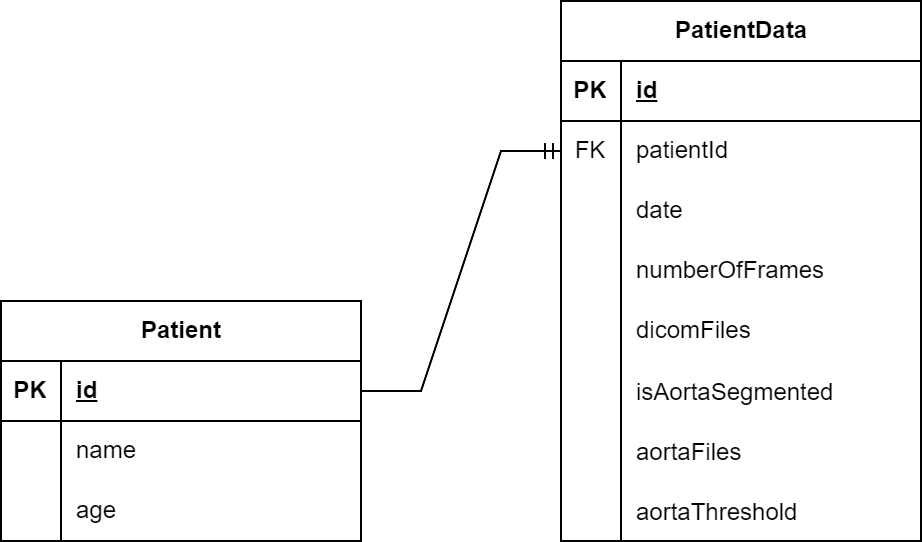
\includegraphics[]{images/chap3/db.drawio.png}
        \caption{Схема базы данных}
        \label{fig:db_scheme}
    \end{figure}
    
В данной схеме база данных состоит из двух таблиц: Patient и PatientData.

\begin{itemize}
    \item таблица Patient содержит основную информацию о пациентах из метаданных;
    \item таблица PatientData предназначена для хранения данных, таких как дата исследования, количество кадров, файлы DICOM, данные сегментации.
\end{itemize}

В будущем планируется модификация данной схемы базы данных для интеграции линий пришиваний и створок клапанов, а также других метаданных пациента при необходимости.

\subsection{Вспомогательные библиотеки для React}

Как было упомянуто в \hyperref[subsec:react]{разделе \ref{subsec:react}}, React сам по себе не является полноценным фреймворком, а скорее библиотекой для создания пользовательских интерфейсов. Для реализации многих ключевых функций требуется использование дополнительных библиотек. В этом разделе мы рассмотрим несколько важных вспомогательных библиотек, которые использовались в проекте.

Для реализации Flux-архитектуры в приложении был выбран Redux. Flux-архитектура помогает управлять состоянием приложения и потоками данных, что особенно важно в больших и сложных приложениях. Redux предоставляет централизованное хранилище для состояния приложения, что позволяет легко управлять состоянием, отслеживать изменения и проводить отладку.

\begin{itemize}
    \item централизованное управление состоянием: Все состояние приложения хранится в одном месте, что упрощает управление и отладку;
    \item предсказуемость: Изменения состояния осуществляются через специальные механизмы, что делает поведение приложения более предсказуемым;
    \item возможность интеграции с различными инструментами: Redux легко интегрируется с различными инструментами для отладки и тестирования.
\end{itemize}

Создание пользовательского интерфейса с нуля может быть трудоемким и времязатратным процессом, особенно когда речь идет о создании стандартных элементов интерфейса, таких как кнопки, списки, панели навигации и т.д. Для упрощения этого процесса была использована библиотека Material-UI.

Material-UI предоставляет набор готовых компонентов, стилизованных в соответствии с принципами Material Design. Это позволяет:

\begin{itemize}
    \item ускорить разработку интерфейса: Использование готовых компонентов экономит время, необходимое на разработку и стилизацию;
    \item обеспечить единый стиль приложения: Все компоненты стилизованы в одном стиле, что делает интерфейс приложения более согласованным и профессиональным;
    \item поддержка и обновления: Material-UI активно поддерживается сообществом разработчиков и регулярно обновляется, что обеспечивает совместимость с новыми версиями React и других инструментов.
\end{itemize}

Эти вспомогательные библиотеки в совокупности с React позволили создать мощный и функциональный веб-интерфейс, который удовлетворяет все текущие потребности проекта и обладает потенциалом для дальнейшего развития и улучшения.

\section{Ключевые моменты реализации}

Далее описаны ключевые моменты, связанные с объединением различных библиотек и инструментов в единую архитектурную систему. Проблема заключалась в необходимости интеграции различных библиотек, таких как React и Three.js, и управления их взаимодействием в рамках единого приложения. Также описаны основные аспекты взаимодействия с серверной частью.

\subsection{Архитектура приложения}

Для создания полноценного веб-приложения необходимо было объединить несколько библиотек, каждая из которых выполняла бы свою специфическую задачу. В нашем случае это React для создания пользовательского интерфейса и Three.js для работы с 3D графикой. Для удобной интеграции Three.js и React существует библиотека React-Three, однако ее использование не было возможно, так как для использования AMI.js нужна версия Three.js 0.99.0, а для React-Three нужна версия Three.js от 0.125.0.

Первоначальной идеей было взять основные подходы из React-Three и реализовать их самостоятельно для нашего приложения, однако возникли трудности.

Парадигма React-Three хорошо подходила для реализации одной сцены или множества независимых сцен, однако у нас все четыре сцены сильно зависели друг от друга, что создавало сложности в реализации такой парадигмы. Работать с изменяемыми объектами в React и Three.js, а также управлять состоянием и взаимодействием между зависимыми сценами, оказалось непросто.

Одной из проблем, с которой пришлось столкнуться при использовании React, является его строгий режим (strict mode). Cтрогий режим важен для разработки, так как помогает отлавливать потенциальные проблемы и побочные эффекты, отрисовывая каждый компонент дважды. Это позволяет React выявить различные ошибки и некорректное поведение на ранних стадиях. Однако использование строгого режима приводило к дублированию некоторых объектов, что создавало проблемы при работе с 3D сценами.

Подход к архитектуре приложения претерпевал значительные изменения на протяжении разработки. В конечном итоге была выбрана парадигма, которая заключалась в инкапсуляции логики работы с 3D сценой и пользовательским интерфейсом. Для их связи был создан удобный API, позволяющий выполнять операции с 3D сценой (например, добавление или удаление элементов) из пользовательского интерфейса.

Основная идея заключалась в инкапсуляции всей логики работы с 3D объектами в специальных классах. Были созданы два ключевых класса: Renderer3D и Renderer2D для работы с трехмерными и двухмерными сценами соответственно. В этих классах реализованы основные методы, такие как создание сцены, добавление и удаление элементов, а также методы для управления сценами и их визуализацией.Как упоминалось ранее в \hyperref[subsec:react]{разделе \ref{subsec:three}}, для создания сцены нужен элемент canvas из HTML. Однако, чтобы сделать эти классы полностью самостоятельными и независимыми от внешних условий при создании, было решено порождать HTML элемент canvas непосредственно внутри класса, вызывая соответствующие функции для создания HTML элементов, а затем вставлять его в компоненты React в нужном месте.

Эти классы включают основные свойства, описывающие сцену, такие как сама сцена, камера, рендерер и прочие элементы. Различия между классами 3D и 2D сцен заключаются в типах используемых камер и проекциях. 

\begin{itemize}
    \item перспективная камера используется для 3D сцены. Это камера, которая имитирует реальное восприятие объектов, так, как они выглядят в реальной жизни;
    \item ортографическая камера используется для 2D сцены. Она отображает ортогональную проекцию предметов на плоскость, где находится камера, что позволяет получать плоские изображения без перспективных искажений.
\end{itemize}

Так как DICOM файлы представляют собой трехмерные объекты, состоящие из множества двумерных снимков, для взаимодействия с ними используется комбинация наложения этих снимков друг на друга, что проецирует 3D картинку. Эти задачи решаются с помощью Stack Helper и Localizer Helper, предоставляемых библиотекой AMI.js.

Поскольку сцены и отображаемые объекты являются тяжелыми и ресурсоемкими, важно было избежать их дублирования. Для этого был применен паттерн Singleton, который гарантировал, что каждая сцена и объект создаются единожды и могут быть использованы повторно в разных частях приложения. Это позволило решить проблему дублирования объектов, возникающую из-за использования strict mode в React.

Схема такой архитектуры показана на диаграмме компонентов \hyperref[fig:bird1]{(Рисунок \ref*{fig:db_scheme})}.

    \begin{figure}[ht]
        \centering
        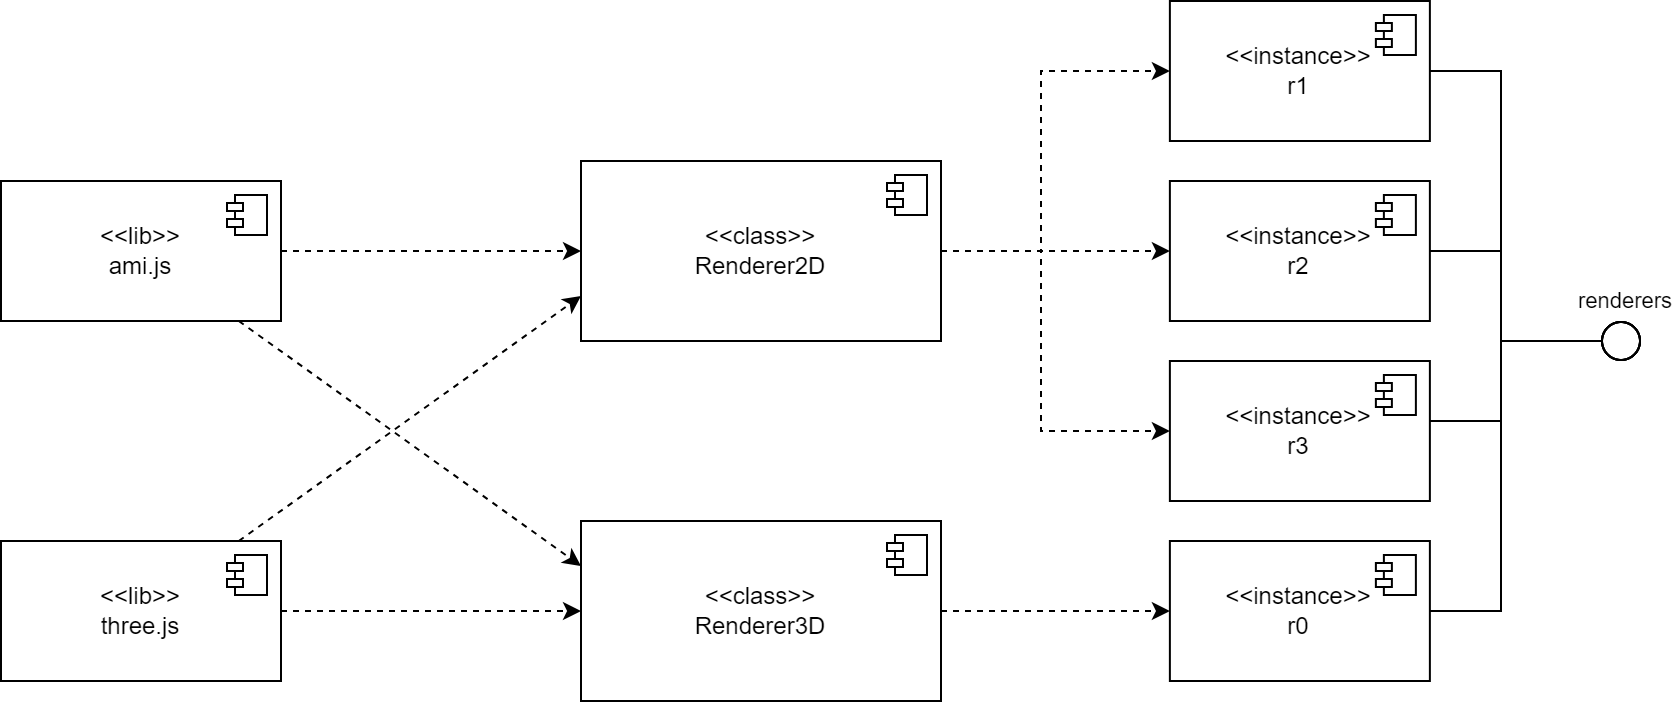
\includegraphics[]{images/chap3/renderers_uml_components.drawio.png}
        \caption{Диаграмма компонентов логики работы с 3D объектами}
        \label{fig:db_scheme}
    \end{figure}

Для удобного доступа к рендерерам в компонентах React были созданы хуки, такие как useRenderer и useRenderers. Эти хуки обеспечивают доступ к рендерерам из любого компонента дерева компонентов, позволяя удобно и эффективно работать с 3D и 2D сценами. Был реализован хук для доступа как ко всем рендерарам, так и к текущему. На \hyperref[fig:hooks]{рисунке \ref*{fig:hooks}} это изображено схематично в диаграмме компонентов.

    \begin{figure}[H]
        \centering
        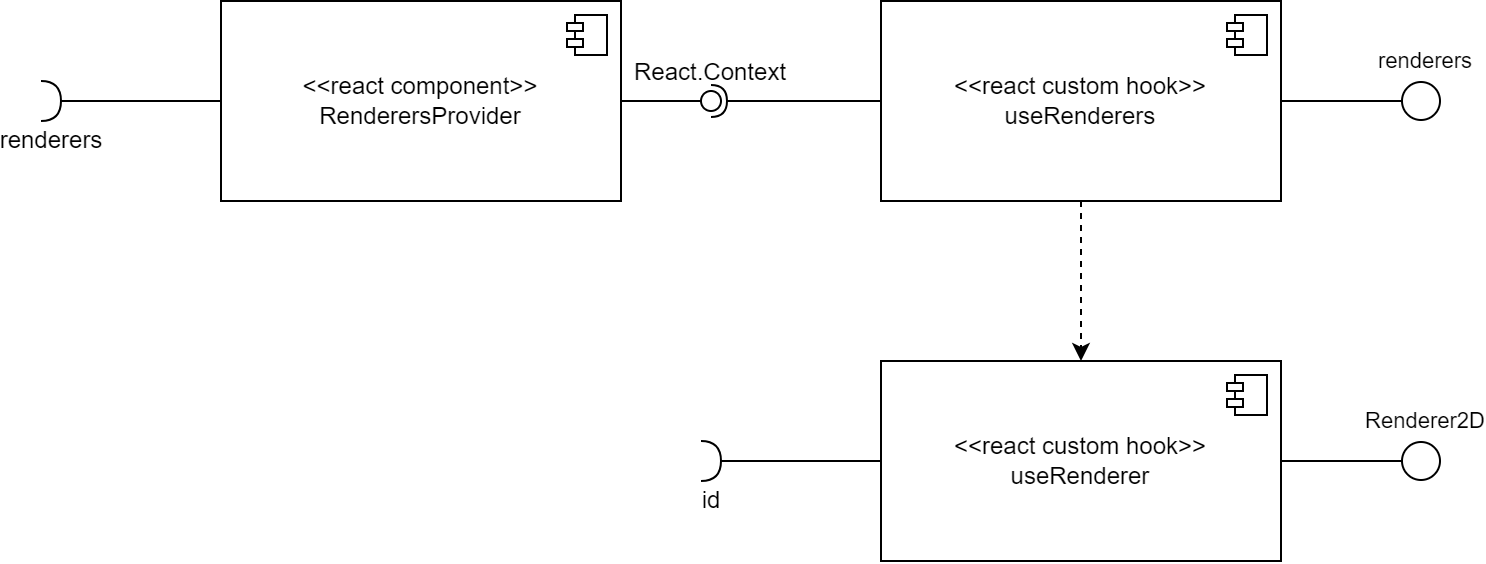
\includegraphics[]{images/chap3/react_uml_components.drawio.png}
        \caption{Диаграмма компонентов доступа рендереров через хуки в UI}
        \label{fig:hooks}
    \end{figure}

\subsection{Компоненты React}

Условно все компоненты можно разделить на три группы:
\begin{itemize}
    \item компоненты, связанные со сценой;
    \item провайдеры;
    \item UI-компоненты.
\end{itemize}

Первые отвечают за инициализацию и управление 3D-сценой, а также за создание и отображение 3D-объектов. Они взаимодействуют с классами Renderer2D и Renderer3D для управления сценами. Список компонентов:
\begin{itemize}
    \item Canvas2D: Компонент для инициализации 2D сцены;
    \item Canvas3D: Компонент для инициализации 3D сцены;
    \item LocalizerHelper: Компонент для работы с локализатором;
    \item StackHelper: Компонент для работы со стеком DICOM;
    \item Aorta: Компонент для отображения сегментированной аорты.
\end{itemize}

Провайдеры обеспечивают управление и доступ к основным элементам системы. Они служат для передачи данных и методов через дерево компонентов, обеспечивая инкапсуляцию и удобное использование ресурсов:
\begin{itemize}
    \item AortaProvider: Обеспечивает доступ к данным сегментированной аорты;
    \item QuadViewProvider: Определяет, какая из сцен используется и управляет четырьмя различными видами;
    \item RenderersProvider: Обеспечивает доступ к классам рендереров для работы с 2D и 3D сценами;
    \item StackProvider: Обеспечивает доступ к DICOM снимкам и управляет их состоянием.
\end{itemize}

UI-компоненты представляют собой элементы пользовательского интерфейса, которые обеспечивают взаимодействие пользователя с системой. Они включают в себя навигационные элементы, списки пациентов и карточки данных пациента:
\begin{itemize}
    \item AppToolbar: Верхняя панель навигации приложения;
    \item AppToolbarButton: Кнопки на верхней панели навигации;
    \item PatientCard: Карточка данных пациента, отображающая информацию о конкретном пациенте;
    \item PatientCardList: Список карточек пациентов, содержащий данные обо всех пациентах;
    \item PatientDataCard: Карточка данных пациента, отображающая информацию о конкретном снимке;
    \item PatientDataCardList: Список карточек данных пациента, содержащий информацию обо всех снимках пациента;
    \item QuadView: Компонент, объединяющий все четыре сцены.
\end{itemize}

\subsection{Взаимодействие с серверной частью}

Общение между клиентом и сервером было реализовано через WebSocket. Для этого было несколько причин:

\begin{itemize}
    \item необходимость отслеживания длительных операций: Процесс выполнения некоторых операций может занимать значительное время. Например, сегментирование аорты выполняется около 30-40 секунд, а моделирование до 3 минут. HTTPS запросы для таких длительных операций неэффективны, так как они не позволяют эффективно отслеживать прогресс и могут приводить к таймаутам. WebSocket позволяет поддерживать постоянное соединение, обеспечивая двустороннюю связь между клиентом и сервером, что позволяет эффективно отслеживать прогресс выполнения операций;
    \item совместимость с Docker-контейнерами: Все решение, включающее все модули, будет упаковано в Docker-контейнер и доступ к серверу и клиенту будет осуществляться с одного и того же домена. Использование HTTPS запросов в данном случае вызывало бы ошибки в браузере из-за политик безопасности, связанных с кросс-доменными запросами. WebSocket позволяет безопасно обходить эти ограничения, обеспечивая надежное взаимодействие между клиентом и сервером;
    \item опыт использования WebSocket в предыдущей версии проекта: взаимодействие с сервером также осуществлялось через WebSocket по аналогичным причинам. Уже была готова некоторая база кода для работы с WebSocket, что облегчило внедрение этой технологии в текущий проект.
\end{itemize}

Было создано API для взаимодействия с сервером, упакованное в отдельный пакет. Это API предоставляет интерфейс для отправки и получения данных через WebSocket. API включает методы для отправки снимков и параметров сегментации (Threshold) на сервер, а также для обработки сообщений, поступающих от сервера. В рамках проекта была проведена работа по реализации типизации для этого API.

Механизм взаимодействия через WebSocket включает следующие шаги:

\begin{enumerate}
    \item Отправка данных на сервер: Клиент отправляет снимки и порог сегментации на сервер через WebSocket.
    \item Обработка сообщений от сервера: Сервер может отправлять сообщения о прогрессе выполнения операции. Когда сервер отправляет сообщение, в API создается искусственное событие.
    \item Подписка на события: на клиенте создается подписка на эти искусственные события с помощью стандартных Event Listener в JavaScript. Например, при получении сообщения о прогрессе сегментации клиент обновляет прогресс бар.
    \item Получение результатов: Когда сервер завершает операцию и отправляет результат (например, STL файл аорты), соответствующее событие срабатывает, и клиент обрабатывает полученные данные.
\end{enumerate}

Схематично взаимодействие сервера и клиента отражено на \hyperref[fig:ws]{рисунке \ref*{fig:ws}}.

\begin{figure}[ht]
    \centering
    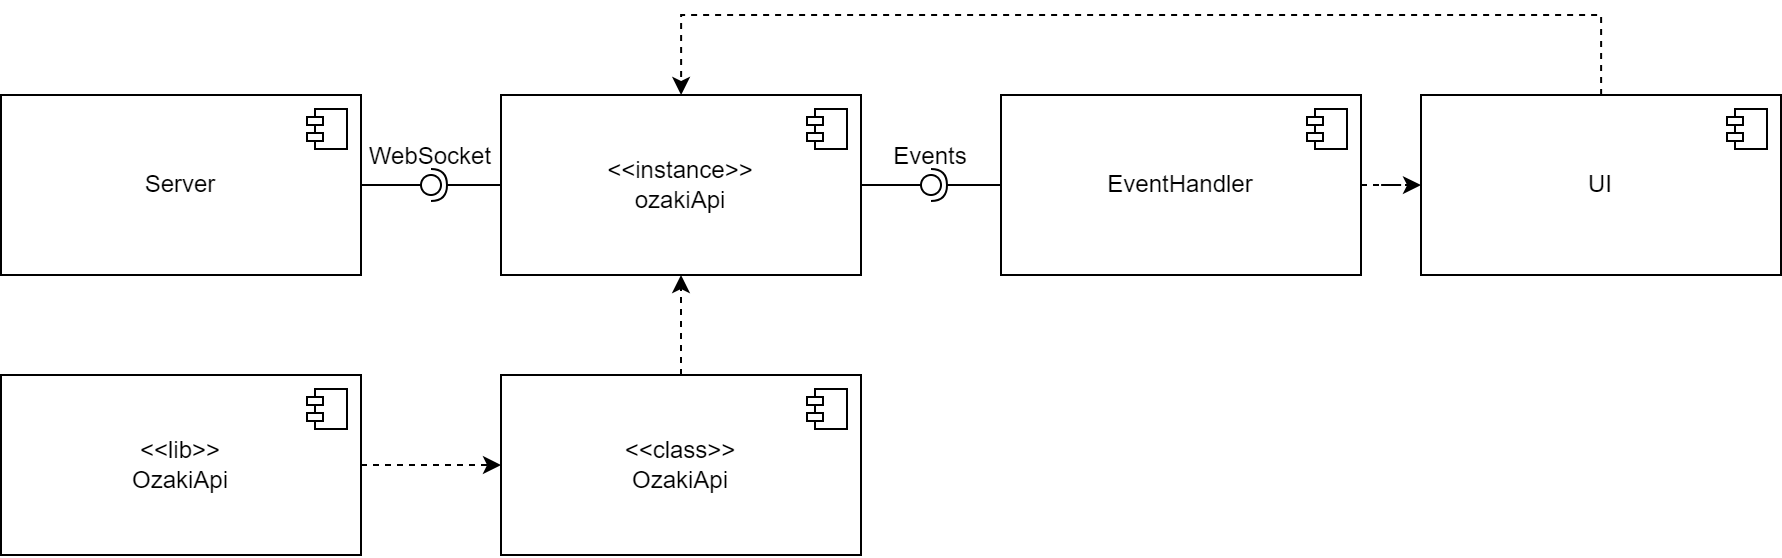
\includegraphics[]{images/chap3/ws_components.drawio.png}
    \caption{Диаграмма компонентов взаимодействия серверной и клиентской части}
    \label{fig:ws}
\end{figure}

STL файл сохраняется в локальную базу данных (Dexie.js) для последующего использования. Для загрузки STL файлов используется модуль Three.js, который обеспечивает визуализацию и дальнейшую работу с 3D моделями.

Таким образом, использование WebSocket для взаимодействия с сервером обеспечило эффективное и надежное выполнение длительных операций, а также позволило реализовать удобный механизм отслеживания прогресса и получения результатов в реальном времени.

Одной из ключевых задач при развертывании клиент-серверного приложения было автоматическое определение URL сервера в production режиме, когда клиент и сервер находятся в одном Docker-контейнере. Для этого была реализована соответствующая функция, которая автоматически определяет URL сервера.

Когда клиентская версия находится в developer режиме, автоматическое определение URL сервера необходимо отключать. В этом режиме удобно вручную вводить нужный URL для тестирования и отладки. Чтобы автоматизировать этот процесс и избежать необходимости ручного переключения URL, использовалась одна из функций сборщика Vite.

Vite позволяет настраивать окружение и переменные окружения, которые фиксируют текущий режим работы (developer или production). В зависимости от режима, в код вставляется соответствующая переменная.

Была настроена система переменных окружения, которая позволяет автоматически переключаться между режимами developer и production. Это существенно упростило процесс разработки и развертывания приложения, так как отпала необходимость вручную править код.

\section{Демонстрация работы приложения}

В этом разделе представлены скриншоты работающего приложения, демонстрирующие основные функции и возможности системы. Визуальные примеры помогают лучше понять, как реализованы и функционируют различные компоненты приложения.

На \hyperref[fig:dicom]{рисунке \ref*{fig:dicom}} показано отображение DICOM снимков на всех четырех сценах. Это позволяет пользователям просматривать снимки пациента в разных проекциях и настраивать параметры визуализации для получения наиболее информативных изображений.

\begin{figure}[h!]
    \centering
    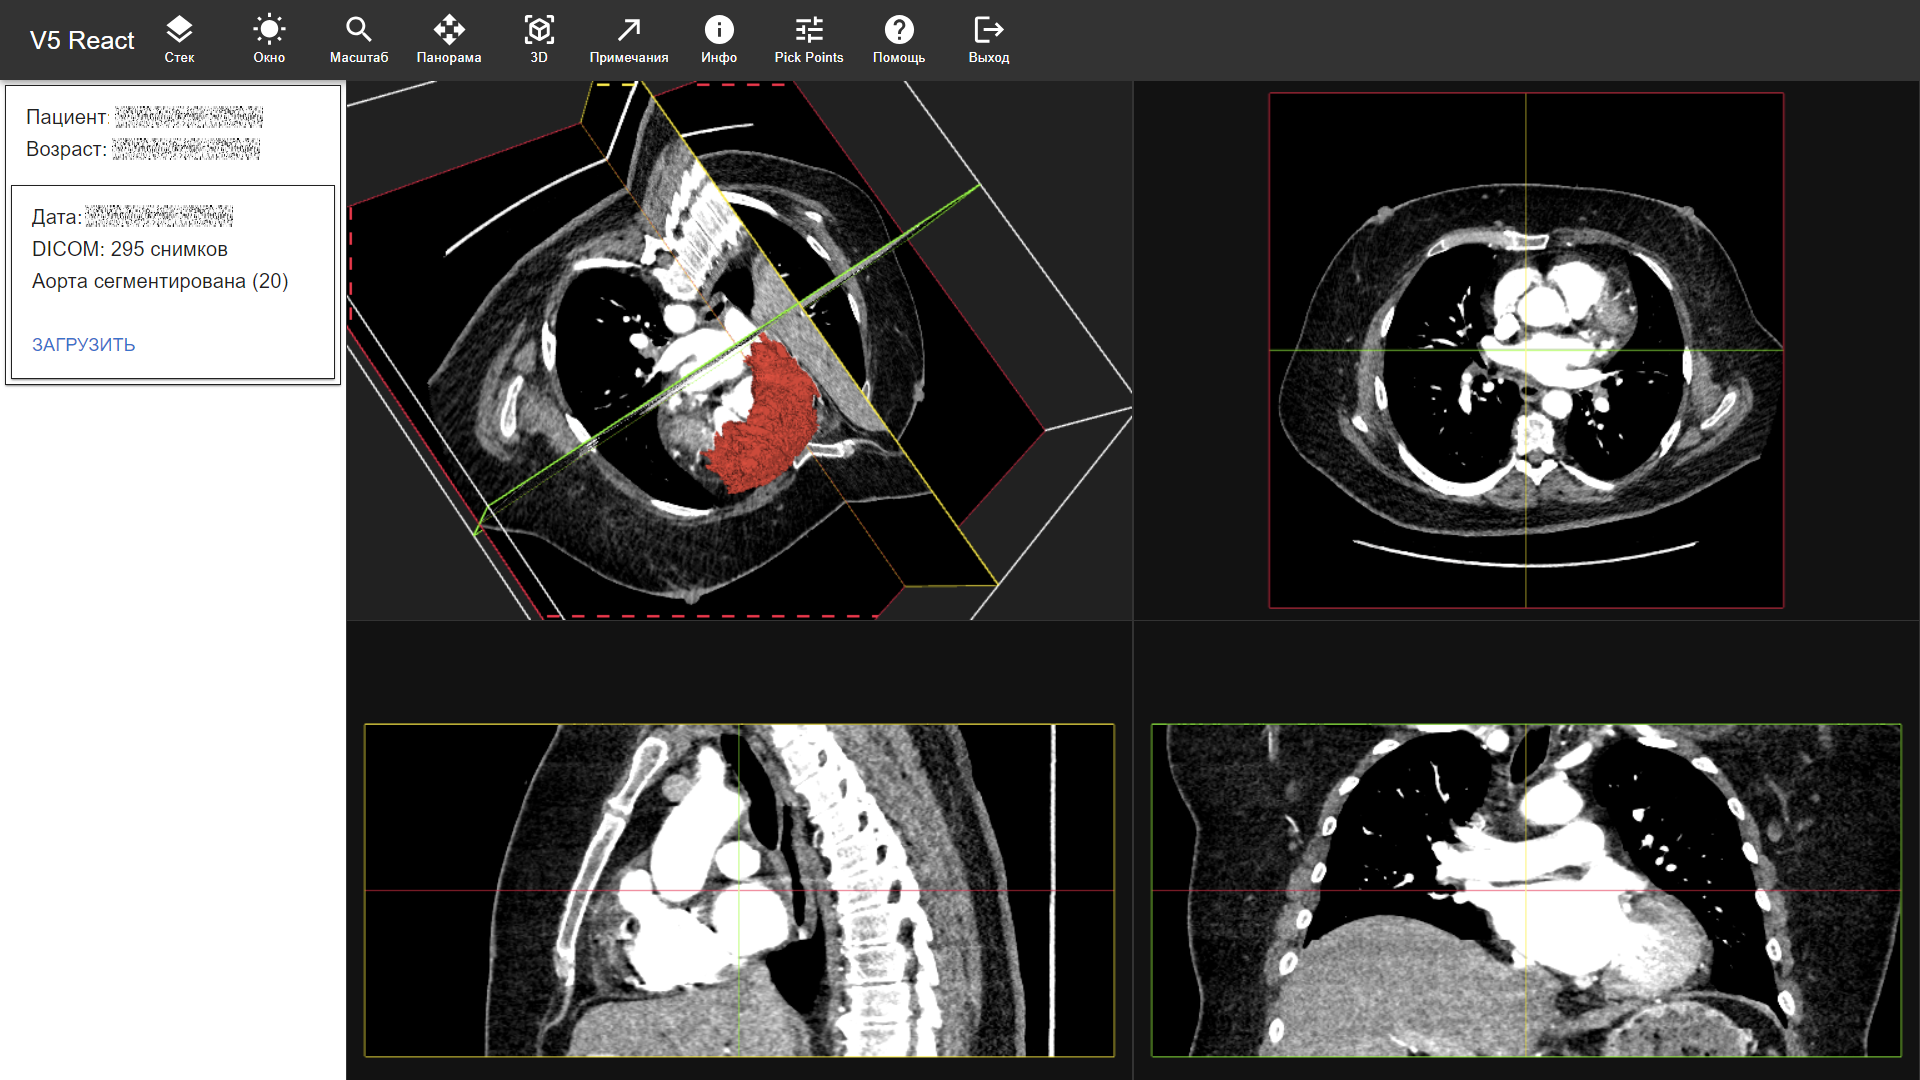
\includegraphics[]{images/chap3/dicom.png}
    \caption{КТ пациента в 3 проекциях}
    \label{fig:dicom}
\end{figure}

На \hyperref[fig:aorta]{рисунке \ref*{fig:aorta}} демонстрируется сегментированная аорта для пациента. Сегментация позволяет выделить аорту на снимках и визуализировать ее в 3D пространстве.

\begin{figure}[H]
    \centering
    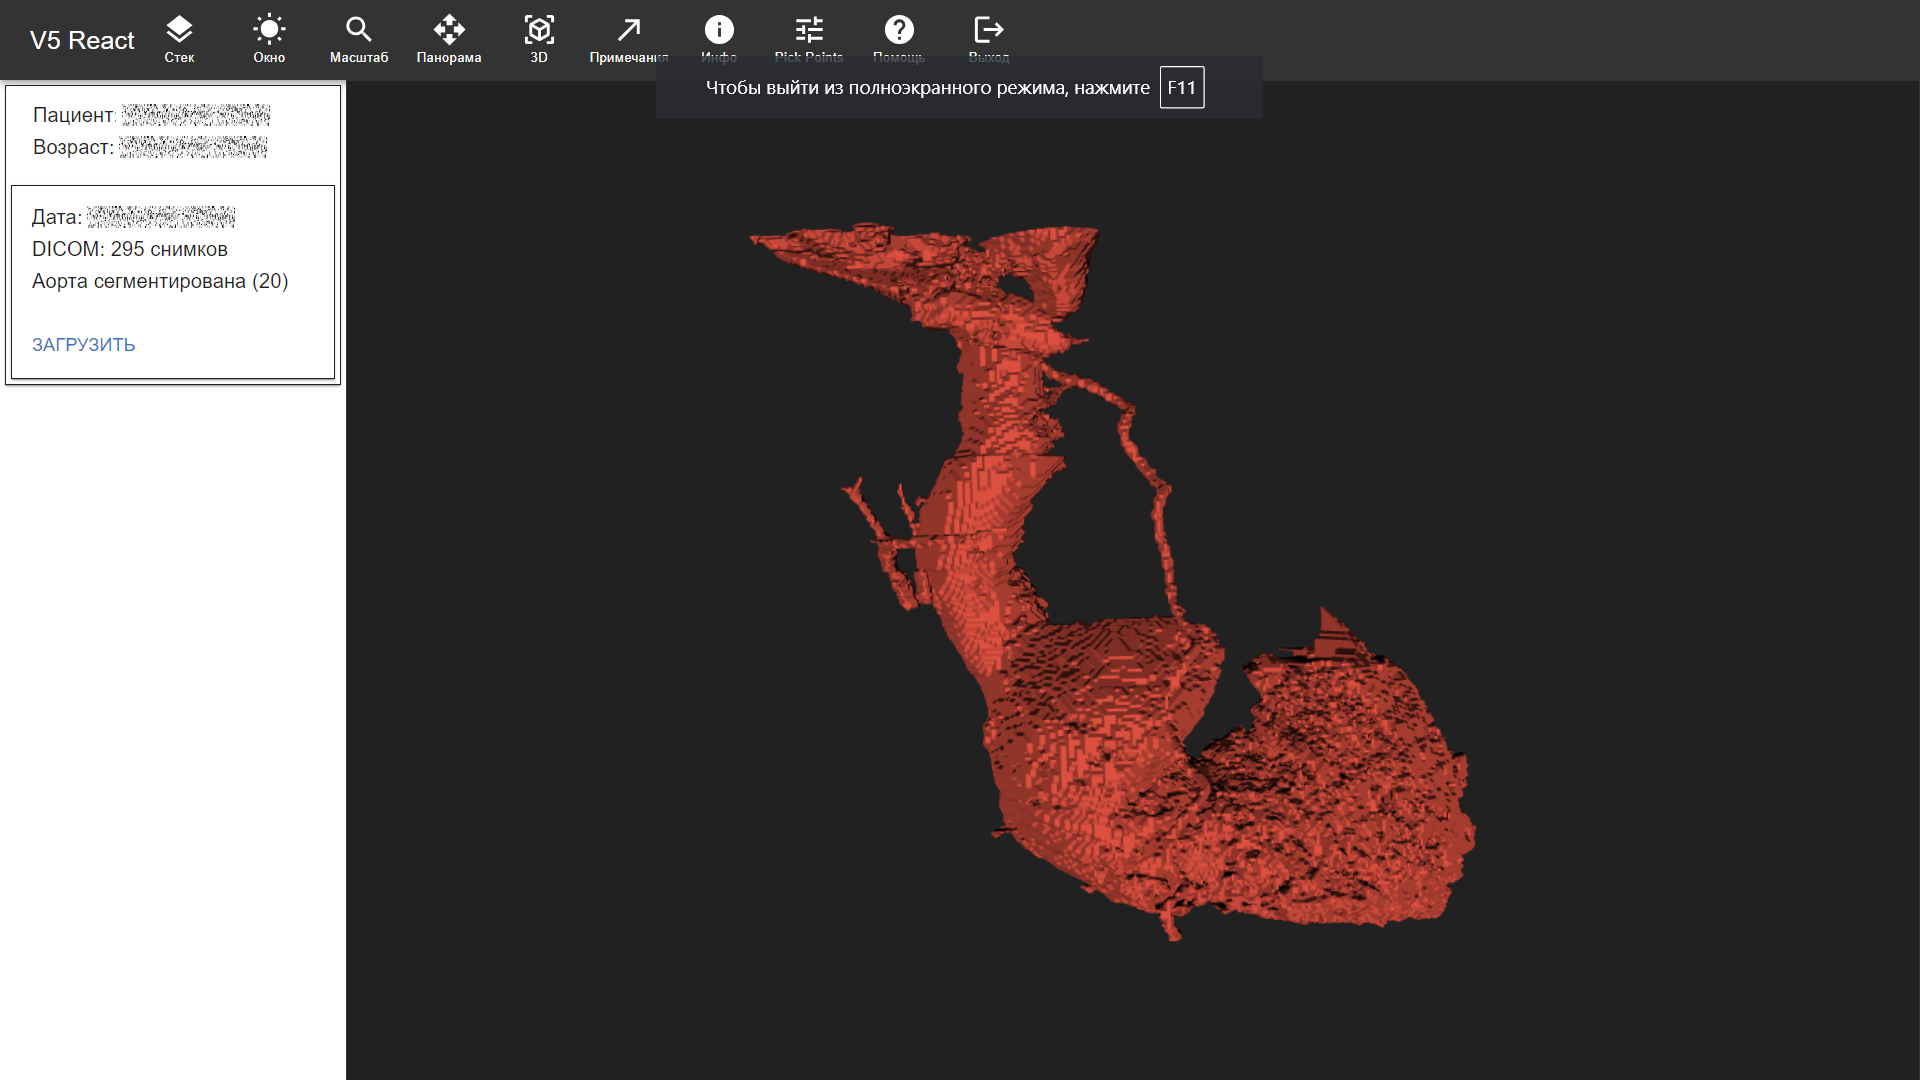
\includegraphics[]{images/chap3/aorta.png}
    \caption{Сегментировная 3D модель аорты}
    \label{fig:aorta}
\end{figure}

На \hyperref[fig:dialog]{рисунке \ref*{fig:dialog}} демонстрируется диалог для сегментации аорты.

\begin{figure}[h!]
    \centering
    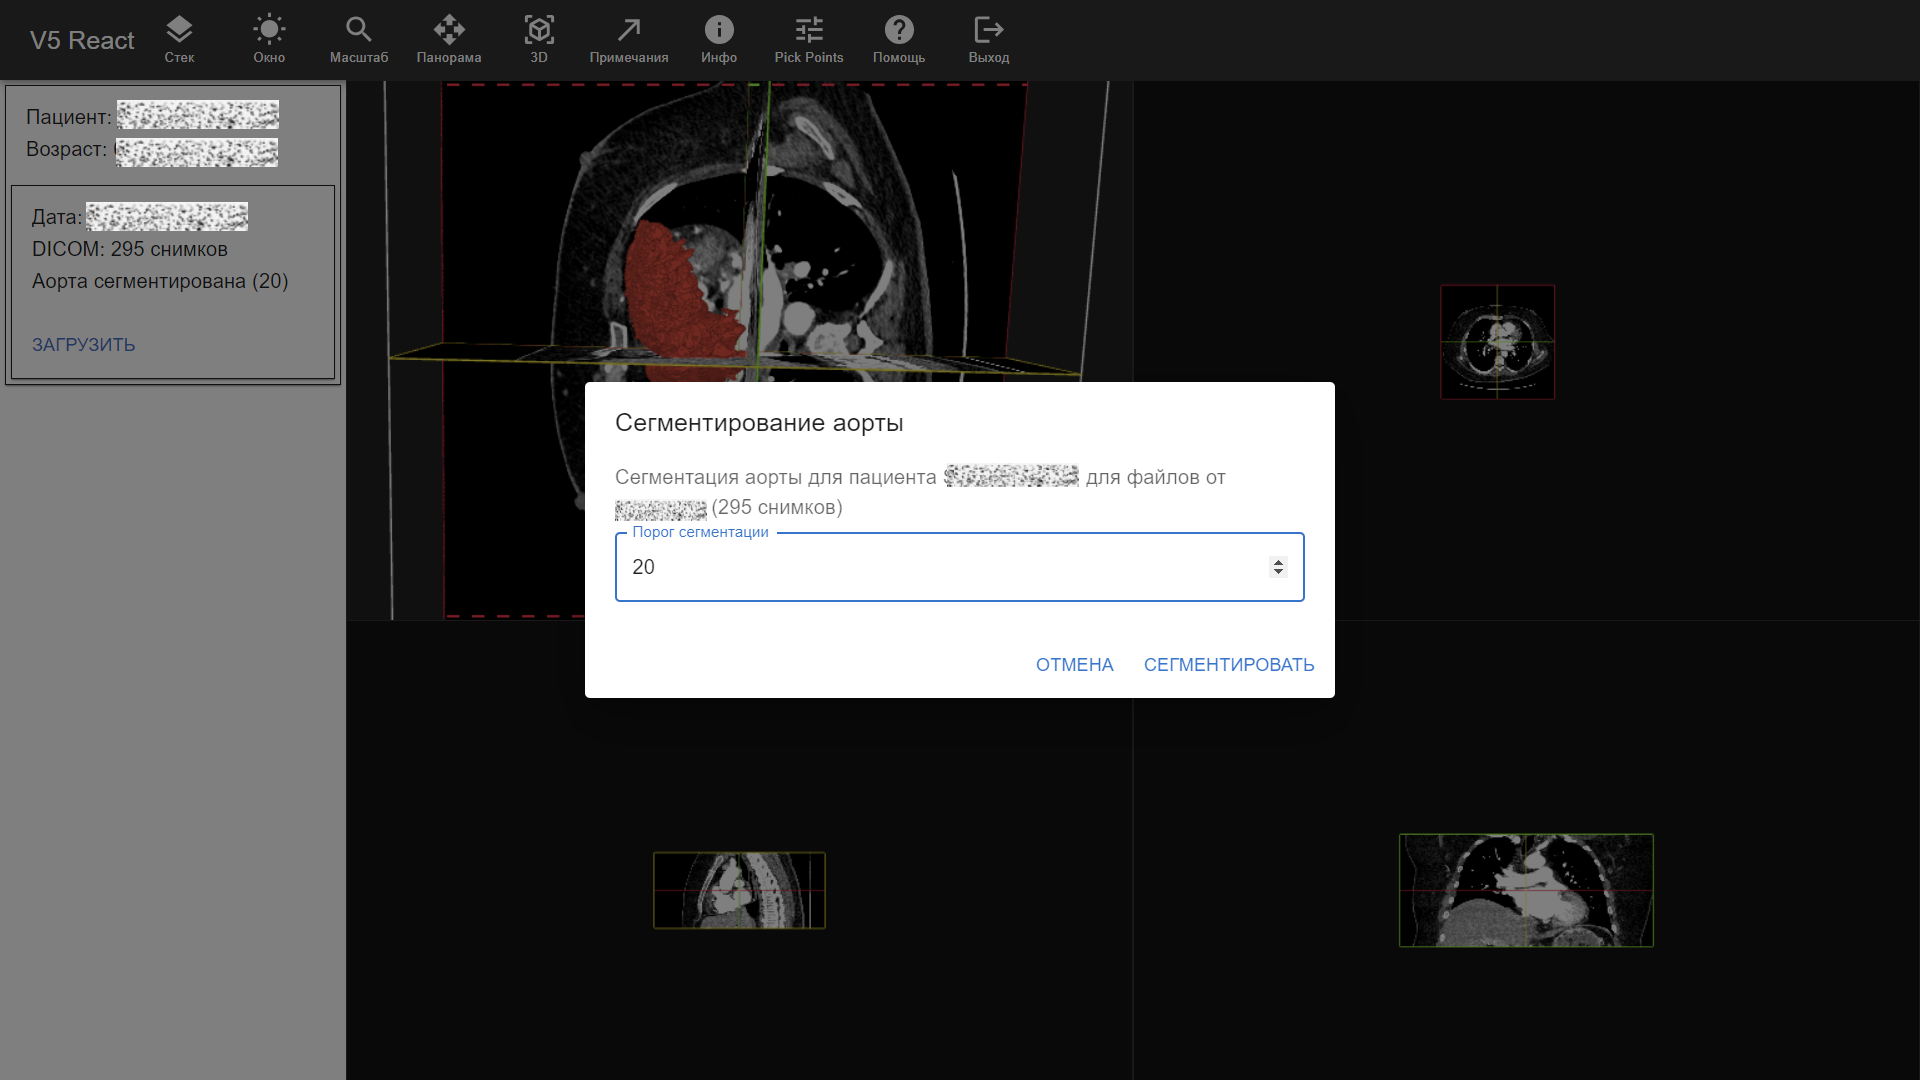
\includegraphics[]{images/chap3/dialog.png}
    \caption{Диалог сегментации аорты}
    \label{fig:dialog}
\end{figure}

На \hyperref[fig:progress]{рисунке \ref*{fig:progress}} демонстрируется отображение прогресса при выполнении сегментации на стороне сервера, что позволяет контролировать и отслеживать выполнение длительных операций.

\begin{figure}[h!]
    \centering
    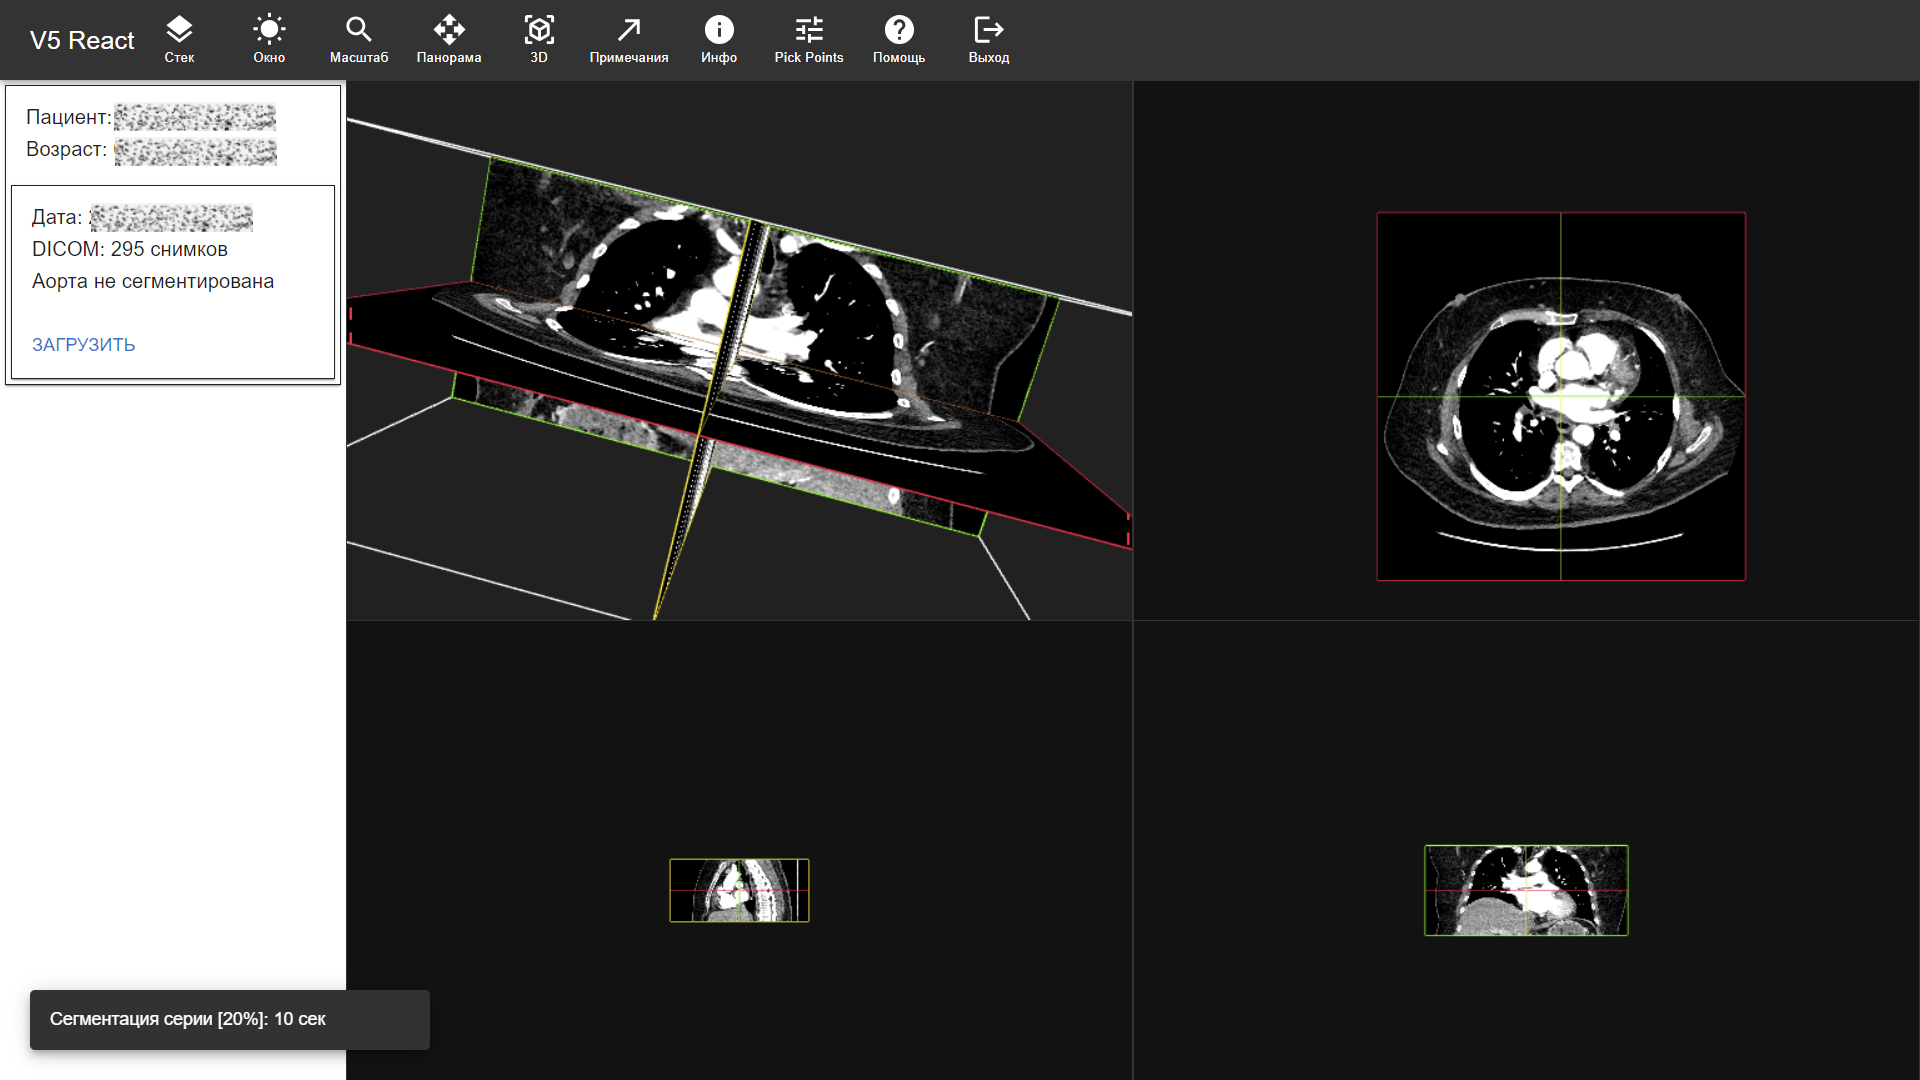
\includegraphics[]{images/chap3/progress.png}
    \caption{Прогресс сегментации}
    \label{fig:progress}
\end{figure}

На данном этапе удалось реализовать только две из четырех основных функций, описанных в разделе \hyperref[subsec:req]{разделе \ref{subsec:req}}. В частности, были разработаны интерфейсы для загрузки данных пациента и их просмотра, а также сегментация и визуализация аорты.

Разработка следующих функций, таких как проведение линий пришивания створок клапана аорты и визуализация результатов моделирования, будет следующим шагом в развитии проекта. Эти функции планируется реализовать в рамках последующих этапов работы.

\endinput                                     % Третья глава
\chapter*{Заключение}

Целью данной работы была разработка пользовательского веб-интерфейса в системе поддержки принятия врачебных решений для операции Озаки с использованием современных фреймворков. В ходе выполнения работы цель была достигнута. Был создан веб-интерфейс, реализующий следующие ключевые функции:

\begin{itemize}
    \item загрузка данных пациента и их просмотр: пользователи могут легко загружать КТ данные пациент в формате DICOM, а также просматривать их, используя основные функции такие как панорамирование, зумирование и вращение изображений.
    \item сегментация и визуализация аорты: обеспечена интеграция с серверной частью для выполнения задач по сегментации аорты и наглядного отображения результатов сегментации.
\end{itemize}

Разработанный веб-интерфейс основывается на современных инструментах, которые были выбраны путем анализа проблем старой кодовой базы и современных подходов к созданию веб-интерфейсов. Интерфейс реализован на языке TypeScript, использует сборщик Vite и фреймворк React. Для работы с 3D-графикой и медицинскими изображениями применяются библиотеки Three.js и Ami.js. Он соответствует современным требованиям и критериям, таким как масштабируемость, развертываемость, поддерживаемость и сопровождаемость.

Работа над проектом будет продолжена в рамках аспирантуры. Вторая часть разработки включает проведение линий пришивания створок клапана аорты, что станет следующим этапом совершенствования системы.

Код проекта доступен на github https://github.com/Micro-ice-ice/v5-react.



\printbibliography[title=Список использованных источников] % Автособираемый список литературы

\end{document}